\documentclass[pdftex,12pt,a4paper]{report}
% \documentclass[pdftex,12pt,a4paper,oneside]{scrbook}
% \documentclass[pdftex,12pt,a4paper]{book}
\usepackage{dbstmpl}
\usepackage{acronymsstyle}

% Hier die eigenen Daten eintragen
\global\arbeit{Master's Thesis}
\global\titel{Detecting Global Correlated Clusters using Hough Transform through Locally Dense Correlations}
\global\bearbeiter{Long Mathias Yan}
\global\betreuer{Daniyal Kazempour}
\global\aufgabensteller{Prof. Dr. Peer Kr"oger}
\global\abgabetermin{19. February 2020}
\global\ort{Munich}
\global\fach{Computer Science}

\begin{document}
\listoftodos 
% Deckblatt
\deckblatt

% Erklaerung fuer das Pruefungsamt
\erklaerung

% Zusammenfassung
\begin{abstract}
Dieses Dokument dient als Muster f"ur die Ausarbeitung einer \the\arbeit\
an der Lehr- und Forschungseinheit f"ur Datenbanksysteme am Institut f"ur
Informatik der LMU M"unchen.
\end{abstract}

% Inhaltsverzeichnis
\tableofcontents

% Hier beginnt der eigentliche Text
% \chapter*{Abbreviations}
\addcontentsline{toc}{chapter}{Abbreviations}
\begin{acronym}
    \acro{OPTICS}[OPTICS]{Ordering Points To Identify the Clustering Structure}
    \acro{ELKI}[ELKI]{Environment for Developing KDD-Applications Supported by Index-Structures}
    \acro{DBSCAN}[DBSCAN]{Density-based spatial clustering of applications with noise}
    \acro{ORCLUS}[ORCLUS]{Arbitrarily ORiented projected CLUSter generation}
    \acro{LMCLUS}[LMCLUS]{Linear Manifold Clustering}
    \acro{4C}[4C]{Computing Correlation Connected Clusters}
    \acro{ERiC}[ERiC]{Exploring Relationships among Correlation clusters}
    \acro{HiCO}[HiCO]{Hierarchical Correlation Ordering}
    \acro{CASH}[CASH]{Clustering in Arbitrary Subspaces based on the Hough transform}
    \acro{D-MASC}[D-MASC]{Dataspace Mean Shift Applied Scan for linear Correlations}
    \acro{ARI}[ARI]{Adjusted Rand Index}
    \acro{NMI}[NMI]{Normalized Mutual Information}
    \acro{hnf}[HNF]{Hesse Normal Form}
    \acro{SUBCLU}[SUBCLU]{density-connected SUBspace CLUstering}
    \acro{CLIQUE}[CLIQUE]{CLustering In QUEst}
    \acrodef{PCA}[PCA]{Principal Component Analysis}
\end{acronym}
\printglossary[type=\acronymtype, style=modsuper, title=List of Acronyms and Abbreviations]
\chapter{Introduction}\label{ch:intro}

In the midst of the fast-paced advancements in data processing and data acquisition, we currently are living in the age of increasing data abundance. While significant improvements in computing power enabled feasible information extraction processes, created the data-centric business practice and opened new possibilities in research in the first place, the concurrent rising acceptance of data collecting technologies and the hunger for more data in hopes for later use, rapidly increased and overtook the processible amount of data. 
% In the midst of the fast-paced advancements in data processing and even faster-paced data acquisition, we currently are living in the world and age of increasing data abundance. While significant improvements in computing power enabled feasible information extraction processes, created the data-centric business practice and opened new possibilities in research in the first place, the concurrent rising acceptance of data collecting technologies and the hunger for more data in hopes for later use, rapidly increased and overtook the processible amount of data. 
%  driven by e.g. increasingly powerful smart devices and other user behaviour tracking practices, increased the amount of data sources rapidly,
%Therefore even with an abundance of data the actual problem of information scarcity still applies.

This raw data often is present in the form of vast amounts of observations consisting of several features represented as numerical values and, thus, is hardly comprehensible for human insight or intuition. Without a 
procedure to extract meaningful information out of the data, this data abundance would be mostly useless for immediate human processing. One way to cope with this issue is the manual labelling of each observation. by human hand, which however obviously is getting more and more unrealistic since with the increasing amounts of data this task is getting inefficient and/or even infeasible. Therefore an automated method to extract relevant information is becoming essential to analyzing the exploding amounts of data. %To tackle this problem, there has been done much research in the fields of Deep- and Unsupervised Learning.

To deal with this problem, there has been lots of different approaches.
If the actual relevant features are not required and are just the means to achieve a goal, the analyzing task can be solved via implicit feature engineering, where it is assumed that the analyzing model learns relevant features by itself.
However if not, the analyzing task can be approached via unsupervised knowledge discovery processes, with goals such as a segmentation of data sets by some shared attributes, a simplification of data sets by aggregating variables with similarity or the detection of anomalies or correlations.

In tasks working with high-dimensional data sets, such as genome analysis in biology/medicine and text analysis in \gls{nlp}, it is particularly interesting, which \textit{features} play important roles in characterizing clusters. This task is called subspace clustering. In the special case of an additional interest in how the important features relate to each other, the task of \textit{correlation clustering} arises.

The problem with existing subspace and correlation clustering approaches is, that they are restricted to a given scope, either local or global, and do not have the capabilities to find the opposite scopes' result. This is inconvenient and limits the thorough evaluation of clusterings if both scopes are of interest. Our goal is to combine existing clustering paradigms to create a correlation clustering algorithm for both scopes simultaneously.

% does not restrict itself to the economic field but is apparent in various fields of science, such as


% This work in particular aims to tackle the
% In this work, we focus on an unsupervised solution for this problem. Namely, we propose a novel algorithm, which combines two different concepts to get a universal clustering of the data.

% \acrfull{cash} is cool, however its complexity is $\mathcal{O}(n^2)$.
% We try to do it better by using a density-based approach to prune away irrelevant points and noise.

\section{Problem Statement}
Our proposal is a correlation clustering algorithm, which builds upon an existing local classical clustering approach and a global correlation clustering approach. It combines those into a more exhaustive algorithm which can give a more comprehensive insight, notably a simultaneously local and global view, onto the applied data while additionally providing a similar performance compared to the global correlation clustering approach. In particular, we first apply a density-based approach onto the data sets to filter out relevant subintervals of the original data space (not to be confused with subspaces) and evaluate those by applying a correlation clustering algorithm based on the Hough transform. Those local results are then stitched together and used to reevaluate previously (falsely) pruned points, to get a complete evaluation of every point of the data set. With this approach, we receive a labelling of a local view and also a global view of the points. 

\section{Structure of the Thesis}
The structure of this thesis is organized as follows:

First off, \textit{\autoref{ch:intro}} introduces/illustrates the motivation of our thesis using tasks/problems from various fields of the current age.
\textit{\hyperref[ch:overview]{Chapter~\ref*{ch:overview}}} gives a general overview of the terminology of clustering, provides a general structure of its different archetypes and leads the reader towards our unique use case.
\textit{\hyperref[sec:Related Work]{Chapter~\ref*{sec:Related Work}}} covers a collection of related works not able to cluster in the desired manner with regards to correlation clustering and introduces components necessary to our algorithm to tackle these problems.
In \textit{\autoref{ch:Methods}}, we provide an in-depth explanation of our algorithm's core components and give an extensive view of the separate steps of our novel approach.
\textit{\hyperref[ch:evaluation]{Chapter~\ref*{ch:evaluation}}} examines our algorithm's runtime, and clustering performance with regards to different data set characteristics, such as numbers of data objects, amount of noise and dimensionality, and compares its result to its ancestor/peer \acrshort{cash}.
To wrap up this work, \textit{\autoref{ch:conclusion}} concludes this thesis by summarizing the current state of research in the field of correlation clustering, and based on the results, aims to categorize our approach within this field. As an outlook \textit{\autoref{ch:futurework}} points out possible future work.

% First off \textit{\autoref{ch:intro}} introduces/illustrates the motivation of our thesis using tasks/problems from various fields, e.g. biology, medicine, economy, etc., of the current age.
% \textit{\hyperref[ch:overview]{Chapter~\ref*{ch:overview}}} gives a general overview of the terminology of clustering, provides a general structure of the different archetypes and leads the reader towards our special type of clustering where our use case is relevant.
% \textit{\hyperref[sec:Related Work]{Chapter~\ref*{sec:Related Work}}} covers a collection of related works not able to cluster in the desired manner with regards to correlation clustering and introduces components necessary to our algorithm to tackle these problems.
% In \textit{\autoref{ch:Methods}} we provide an in depth explanation of our algorithms core components and give an extensive view to the separate steps of our novel approach.
% \textit{\hyperref[ch:evaluation]{Chapter~\ref*{ch:evaluation}}} examines our algorithms runtime and clustering performance with regards to different data set characteristics, such as numbers of data objects, amount of noise and dimensionality, and compares its result to its ancestor/peer \acrshort{cash}.
% To wrap up this work \textit{\autoref{ch:conclusion}} concludes this thesis by summarizing the current state of research in the field of correlation clustering, and based on the results, aims to categorize our approach within this field. As an outlook \textit{\autoref{ch:futurework}} points out possible future work.

% Note that in this thesis \textit{subspaces} and \textit{subspace clusters}, except in \autoref{sec:clu} or unless explicitly stated, always refer to \textit{linear} arbitrarily oriented subspaces/correlations and its clusters. We also use \textit{subspace clustering} and \textit{correlation clustering} interchangeably.
% \todor{Notiz behalten?}
\chapter{Fundamentals}
%evtl. in related work als Einleitende subsections

This chapter briefly gives an overview of the terminology in clustering and mentions a variety of existing clustering algorithms to give a basic understanding of the different tasks/types. Additionally we give insights into some of its relevant branches for the sake of this work, which will be further elaborated in \autoref{sec:Related Work} and \autoref{ch:Methods}. For an indepth explanation of the mentioned algorithms we refer to its respective references.

\section{Clustering}\label{sec:clu}
% Clustering is an unsupervised machine learning/exploratory data mining task and is the process of grouping a set of data objects into groups of \textit{similar} objects. The keyword \textit{``similar''} is dependent on the objective goal of the clustering which is dependent on the task and could demand similar attributes, e.g. finding similar data points, or similar relationships, e.g. data points following a trend. Formally one could state:
% Given data objects $o_i, i\in\{1,2,...,n\}$ with a set of attributes $a_j, j\in\{1,2,...,d\}$. Our data set $ds$ is a set of data objects $ds=\{o_1, o_2, ... , o_n\}$ with $n$ observations which respectively have $d$ Dimensions/attributes. $f$ is a function which Clustering is the optimization problem of minimizing a function $f$ which simply
% These clustering approaches are based on the \textit{locality assumption}

\begin{figure}
    \centering
    \makebox[\textwidth][c]{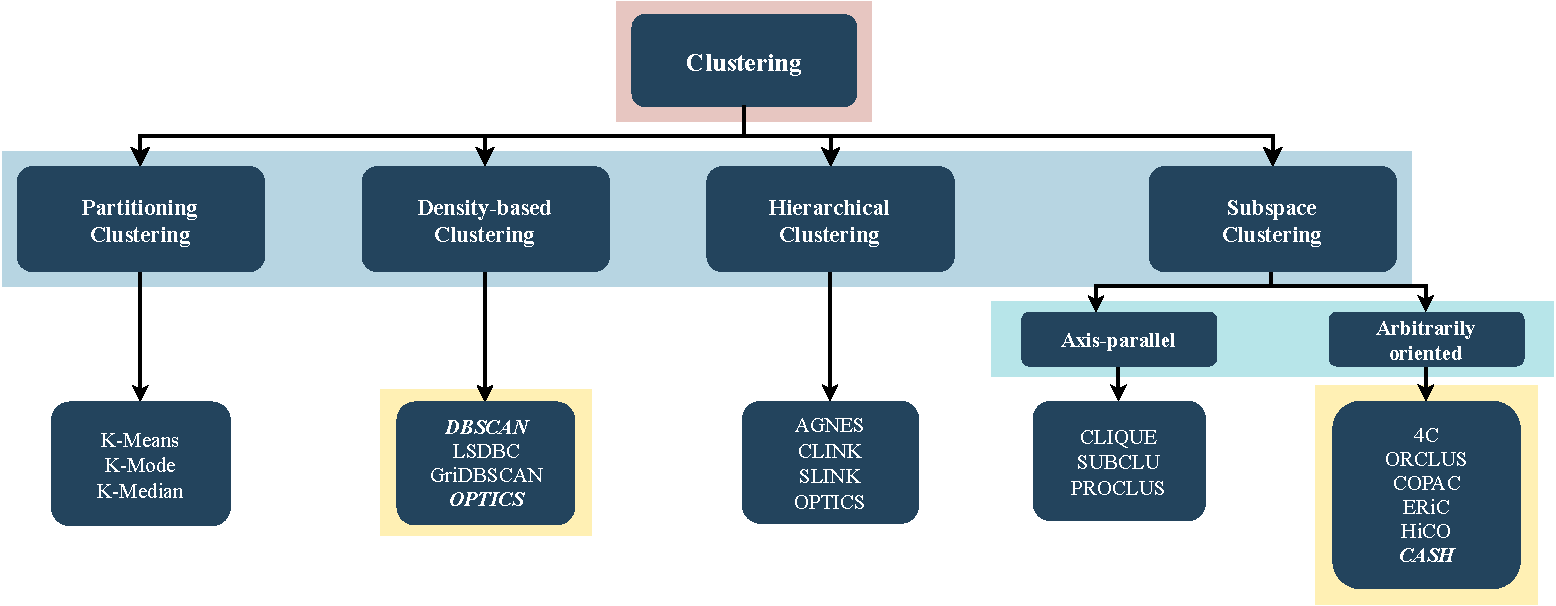
\includegraphics[width=1.1\textwidth, page=1]{figures/ClusteringAxis.pdf}}
    \caption{Topology of Clustering, Yellow marked areas are the main focus of the thesis}
    \label{fig:my_label}
\end{figure}

% source für 'basic verfahren' http://myweb.sabanciuniv.edu/rdehkharghani/files/2016/02/The-Morgan-Kaufmann-Series-in-Data-Management-Systems-Jiawei-Han-Micheline-Kamber-Jian-Pei-Data-Mining.-Concepts-and-Techniques-3rd-Edition-Morgan-Kaufmann-2011.pdf 
% source für subspace clustering verfahren: https://onlinelibrary-wiley-com.emedien.ub.uni-muenchen.de/doi/abs/10.1002/widm.1057
% lmu bookmarklet: https://www.ub.uni-muenchen.de/ausleihe-online/e-medien-login/index.html

% \section{The locality assumption}
\section{Subspace Clustering}\label{sec:subspaceclu}

\chapter{Related Work}
\label{sec:Related Work}
% This chapter introduces some foundational work on density-based and subspace/correlation clustering and aims to give an intuitive insight into existing approaches to solve the problem of subspace clustering. We also elaborate, where these existing approaches lack in ability and capability and show some of the current optimization approaches.
This chapter introduces some foundational work on subspace/correlation clustering and aims to give an intuitive insight into existing approaches to solve the problem of subspace clustering. In particular the elaboration on the related work is twofold: we introduce subspace/correlation extraction/clustering methods such as basic \acrshort{pca} and \acrshort{orclus}, and additionally expand on algorithms which augment the subspace clustering method such as \acrshort{dbscan} in \acrshort{4c}. We also elaborate, where these existing approaches lack in ability and capability and show some of the current optimization approaches.

Since sections \nameref{sec:houghintro}, \nameref{sec:cashintro}, \nameref{sec:dbscanintro} and \nameref{sec:OPTICSintro} are essential components to our work they will be elaborated in greater detail in the chapter \nameref{sec:Foundations}

\section{Existing Subspace Clustering Algorithms}
There are many approaches for detecting relevant subspaces in data, generally grouped to either finding axis-parallel or arbitrarily oriented subspaces. Our work in particular focuses on the extraction of the second type of subspaces, which obviously proves to be a more challenging task since it encompasses the problem of axis-parallel subspace clustering\todor{the first type}. This task is also referred to as \textit{Correlation Clustering}. 

This section introduces some existing correlation clustering algorithms and illustrates \todor{choose one: demonstrates/analyzes/explains/illustrates/points out} their advantages and disadvantages and elaborates on their suitability for our idea.

\subsection{PCA}
A common way to filter out relevant features/subspaces in high dimensional data is the application of feature selection/dimensionality reduction. One of the oldest and most widely used methods is the \gls{pca}. It is a statistical approach which uses an orthogonal transformation to transform the original basis of a $d$-dimensional data space $DS$ to a basis built upon $d$ so called \textit{Principal Components} $PC$, where the first Principal Components $PC_1$ is a vector which describes the largest percentage of explained variance in $DS$. Each Principal Component $PC_j$ next in order $j,\dotsc,d$ is orthogonal to the previous ones $PC_i, i<j$ and is ordered by the next highest explained variance. Mathematically finding the Principal Components in a data set $DS$ boils down to solving its eigendecomposition \todor{nicht ganz korrekt. eigendecomp von cov(x)}, where the eigenvector with the highest corresponding eigenvalue represents the first Principal Component and the second highest the second Principal Component, etc\cite{pcawold1987principal}. For further details to the calculation \textcite{pcamljolliffe1986principal} offers a short and intuitive step-by-step explanation.
Unfortunately the extraction of relevant features via \gls{pca} is rarely of use for clustering problems. Unmodified \gls{pca} is global in nature and can only compute one subspace of the original data space and does not address the problem of \textit{local feature relevance} or \textit{local feature correlation}, which essentially states, that different clusters in data space can exist in different subspaces\cite{kriegel2009clustering} (c.f. \cite{PCAshlens2014tutorial}). \todor{PCA besser erklaeren}

\todob{PCA own fig}
\begin{figure}
    \centering
    \begin{minipage}[t]{.5\textwidth}
      \centering  
      \captionsetup{width=.9\linewidth}
      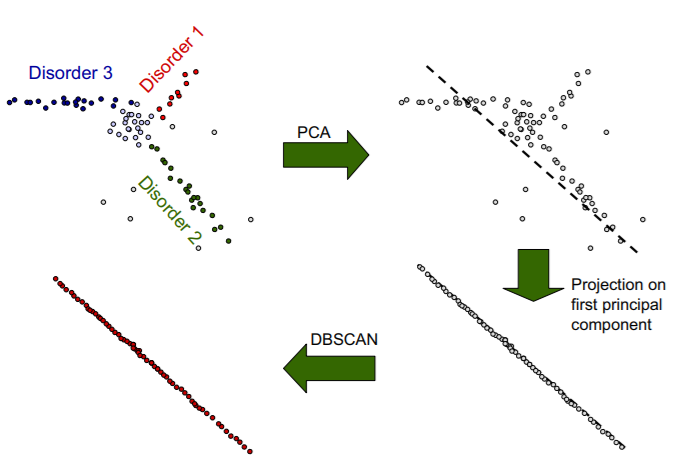
\includegraphics[width=.9\textwidth]{figures/pcalocalfeat1.png}
      \captionof*{figure}{a) First}
      \label{fig:test1}
    \end{minipage}%
    \begin{minipage}[t]{.5\textwidth}
      \centering
      \captionsetup{width=.9\linewidth}
      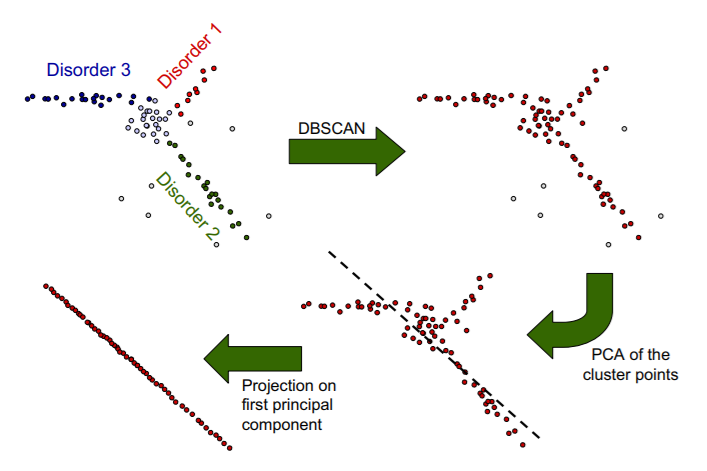
\includegraphics[width=.9\textwidth]{figures/pcalocalfeat2.png}
      \captionof*{figure}{b) Second}
      \label{fig:test2}
    \end{minipage}
    \caption{lazy}
    \label{fig:localfeatrelevance}
\end{figure}

\subsection{ORCLUS}
Since \gls{pca} only provides a global view of the correlations in data space and does not address the local feature relevance, \gls{orclus} attempts to enforce \gls{pca} to only consider local segments of the data space via a $k$-Means-like approach. 

To find $k$ many $l$-dimensional subspace clusters in a $d$-dimensional data space, \gls{orclus} first initializes $k_c, k_c > k$ seeds $s_i$ as centroids and applies the default (euclidean) $k$-Means to partition the data space into $k_c$ clusters $C_i$ with $i \in \{1,\dotsc,k_c\}$. After that iteratively all points are reassigned to the new cluster centroids via a modified distance function based on a subset of $l_c, l\leq l_c \leq d$ weak eigenvectors/principal components $\varepsilon_i$ of each cluster $c_i$. This subset of $l_c$ eigenvectors represents the current dimensionality of the cluster in each iteration and is adapted such that at the end of all iterations $l_c=l$ holds. Additionally at the end of each iteration the closest pair (in terms of average modified distance) of clusters are merged together resulting in $k_c = k_c-1$ clusters afterwards. This reassigning-merging process is repeated until $k_c = k$ holds. Due to the localized view on the single partitions \gls{orclus} is considered as a local correlation clustering algorithm\cite{orclusaggarwal2000finding}.

As an adopter of $k$-Means and \gls{pca}, \gls{orclus} however also comes with its components disadvantages. It relies on $k$, which is difficult to determine, does not handle noise and outliers, and extracts the subspaces based on the clusters eigenvectors, which are not necessarily a good representation of the members distribution (c.f. \autoref{fig:localfeatrelevance}).


\subsection{4C}\label{ssec:4c}
Analogous to \gls{orclus}, \gls{4c} also aims to construct a localized view of the data space. This time however a density-based approach is used. 

To find $\lambda$-dimensional subspace clusters in a $d$-dimensional space, \gls{4c} employs a customized/an extended \acrshort{dbscan} by modifying parts of the density criterion. 
% After clustering the data space into usual dense clusters, each cluster is reevaluated according to its variance. This is done by applying \gls{pca} to the locally dense cluster. If the $d-\lambda$ smallest eigenvectors of the cluster are not close enough to threshold $\delta \approx 0$
Instead of uniformly assessing the neighborhood in all directions, the modified density criterion biases the neighborhood query according to the neighborhoods variance. First, only dense candidates/core points, that have a maximum of $\lambda$ eigenvalues $\varepsilon_i > \delta$ in its neighborhood, are considered. $\delta$ denotes a threshold for a variance in unrelated dimensions. Secondly, these points are grouped together based on their membership in each others modified neighborhood. These resulting clusters are, much like \gls{orclus}, also based on a localized view (this time dense clusters) and therefore also only able to create a local correlation clustering\cite{4cbohm2004computing}. A detailed explanation to the original \acrshort{dbscan} is found in \autoref{ssec:DBSCANindepth}.

In contrast to \gls{orclus}, \gls{4c} enables the handling of noise and outliers. The modification of the density criterion essentially promotes a density-based propagation of the cluster biased towards the found local correlations, but due to the lose constraint of a maximum amount of eigenvalues, \gls{4c} just finds close to $lambda$-dimensional clusters.

\subsection{COPAC}
\gls{copac}, like \gls{4c}, also uses an approach based on \acrshort{dbscan}, however this time the modified \acrshort{dbscan} artificially only considers distances related to the correlating (global) hyperplane and thus creates a global correlation clustering. 

Instead of determining each points dimensionality according to its dense neighborhood (c.f. \autoref{ssec:4c}), \gls{copac} first assigns each point its \textit{local correlation dimensionality} $\lambda$, which denotes the smallest amount of eigenvectors explaining at least $\alpha$ percent of the $k$-nearest neighbors variance, and partitions them based on $\lambda$. Secondly, clusters each partition is processed with a modified \acrshort{dbscan}. This modified \acrshort{dbscan} now only considers the $d-\lambda$ weakest eigenvectors of the k-nearest neighbors in the distance functions and therefore clusters each partition based on the distance to the strong eigenvectors/correlations.

Due to the inital partitioning based on the local correlation dimensionality $\lambda$, \gls{copac} does not need a parameter to detect a specific dimensional correlation, but instead simultaneously finds correlation clusters of arbitrary dimensions. The difficulties here rely on the choice of the parameter $k$, which at least can be constraint to $k>d$
\todor{moechte eigtl nicht sagen, dass das gut oder schlecht ist, vllt will man ja gezielt nach einer dimensionalitaet suchen?}\\


% \subsection{HiCO and ERiC} \todor{passt so halb rein, bau ja n fulldim hierarchy}
% (Global) Correlation Clustering, other algorithms so far (ORCLUS \cite{orclusaggarwal2000finding}, LMCLUS \cite{}, 4C, HiCO, ERiC)[1]

% Since many of the existing correlation clustering algorithms rely on \gls{pca} they also come with its limitations. 

\section{Hough Transformation}\label{sec:houghintro}
The Hough Transform originally was introduced by \textcite{houghOriginal1962method} and extended by \textcite{rosenfeld1969picture} in the field of computer vision for edge detection\cite{houghhistoryhart2009hough}. The initial purpose of the Hough transform was a technique to detect colinear points in an image space but has since then found various other applications in fields like image processing/analysis~\cite{rosenfeld1969picture,ballard1981generalizing}, computer vision~\cite{davies2004machine} and subspace clustering\cite{CASHachtert2008robust}.

The basic idea of the Hough transform is the transformation of all points $p_i = (x_i,y_i)$ in a 2-dimensional image space $\mathcal{D} \subseteq \R^2$ to functions $f_{p_i}$ in a 2-dimensional parameter space $\mathcal{P} \subseteq \R^2$, also known as Hough space\cite{illingworth1988survey}. This is can be done by e.g. taking a representation of a point $p$ as all of its concurrent lines $y_p = m \cdot x_p + t$ and rearranging it to $m_{p} = - \frac{1}{x_p} \cdot t_{p} + \frac{y_p}{x_p}$ which produces a straight with slope $m$ and y-intersect $t$ in a $(m,t)$-parameter space. Since each point in parameter space represents a particular $(m,t)$-setting, multiple functions close to each other implies that their respective points have similar $(m,t)$-settings as well. The correlation clustering objective therefore transforms to a density-based clustering objective in parameter space, with the added benefit of being able to detect correlating points regardless of their distance to each other in data space. This property is exploited by e.g. evaluating the whole parameter space in a grid with a voting scheme or by smartly splitting the parameter space in \autoref{sec:houghintro} to detect linear correlations. 
\todor{Ich plagiere mich selbst. 1zu1 aus unterem abschnitt}
% \begin{figure}
%     \centering
%     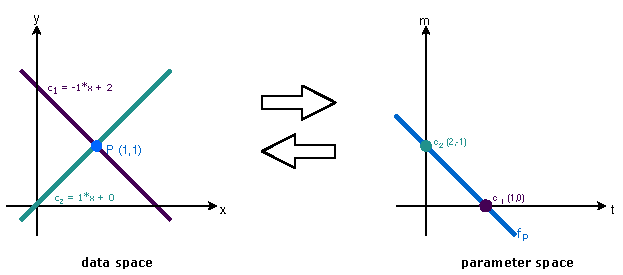
\includegraphics{figures/HoughMXT.pdf}
%     \caption{Caption}
%     \label{fig:houghmxt}
% \end{figure}\todor{eher keine bilder in related work}

\section{CASH}\label{sec:cashintro}
The global correlation clustering algorithm \gls{cash} extends the use case of the Hough Transformation to the detection of arbitrary-dimensional subspaces by augmenting the initial rigid 2-dimensional definition to a multi-dimensional one. 

Furthermore \gls{cash} introduces a improved search strategy for detecting regions of high intersections in parameter space to improve the efficiency compared to the basic grid search \cite{CASHachtert2008global}. Instead of doing an extensive count operation/accumulation of intersections over a fixed interval, \gls{cash} successively splits the whole parameter space by its axes and only further evaluates the split hypercuboids if they contain enough intersections. This is repeated until a certain count of splits is reached and only then hypercuboids with enough intersections are considered as linear correlations. 

Since our work focuses on ``\textit{Detecting Global Correlated Clusters using Hough Transform through Locally Dense Correlations}'', we use \gls{cash} to cope with multi-dimensional data and detect our locally dense correlations. Additionally we will use \gls{cash} as a performance baseline for our descendant algorithm to compare them in a global setting.
A more profound explanation to the transformation and its usage in \gls{cash} will be given in \autoref{ssec:houghindepth}.

% Please add the following required packages to your document preamble:
% \usepackage{booktabs}
% \usepackage{graphicx}
\begin{table}[]
\centering
\resizebox{\textwidth}{!}{%
\begin{tabular}{@{}|l|c|c|c|l|@{}}
\toprule
\textbf{Algorithm}                 & \textbf{\begin{tabular}[c]{@{}c@{}}Local \\ Subspaces\end{tabular}} & \textbf{\begin{tabular}[c]{@{}c@{}}Global \\ Subspaces\end{tabular}} & \textbf{\begin{tabular}[c]{@{}c@{}}Global \\ Subspaces\end{tabular}} & \textbf{Notes}                                                                                                                                                                                                   \\ \midrule
\acrshort{pca}    & \xmark    & \cmark     & \xmark      & \tabitem Only handles single or orthogonal correlations well                                                                                                                                                              \\ \midrule
\acrshort{orclus} & \cmark    & \xmark     & \xmark      & \tabitem Combines \acrshort{pca} with a $k$-Means-like approach                                                                                                                                          \\ \midrule
\acrshort{4c}     & \cmark    & \xmark     & \xmark      & \tabitem Combines \acrshort{pca} with a density-based approach                                                                                                                                           \\ \midrule
\acrshort{copac}  & \xmark    & \cmark     & \xmark      & \begin{tabular}[c]{@{}l@{}}\tabitem Similar to \acrshort{4c}\\ \tabitem Combines \acrshort{pca} with a density-based approach\end{tabular}                                                       \\ \midrule
\acrshort{hico}   & \xmark    & \cmark     & \cmark      & \begin{tabular}[c]{@{}l@{}}\tabitem Creates a Correlation distance ordering similar to \acrshort{optics},\\ \tabitem creates a tree-like hierarchy\end{tabular}                                                   \\ \midrule
\acrshort{eric}   & \xmark    & \cmark     & \cmark      & \begin{tabular}[c]{@{}l@{}}\tabitem Similar to \acrshort{hico}\\ \tabitem Creates a Correlation distance ordering similar to \acrshort{optics}, \\ \quad \ but creates a graph-like hierarchy\end{tabular} \\ \midrule
\acrshort{cash}   & \xmark    & \cmark     & \cmark      & \tabitem Uses the Hough-Transform to                                                                                                                                                                                      \\ \bottomrule
\end{tabular}%
}
\caption{}
\label{tab:corrcluchar}
\end{table}

\section{DBSCAN}\label{sec:dbscanintro}
\citeauthor{DBSCANEKSX96} created a foundational algorithm with \gls{dbscan}. With over 16000 citations on google scholar as of December 2019 it is one of the most influential works created in the field of density-based clustering and a basis to many clustering approaches, not only restricted to density-based clustering. 

As its name reveals it is an algorithm which detects points in dense vicinity and groups them together. For a measure of density \gls{dbscan} utilizes two parameters. One to specify the minimum amount of neighboring points in a close vicinity and one to specify the range/radius of that vicinity. Points fulfilling these conditions are called \textit{core points} and represent the dense \textit{core} of a cluster. The border of a dense cluster is composed of \textit{border points}. They are points which themselves do not possess a dense neighborhood but are still in the vicinity of core points. 

In contrast to $k$-means-like partitioning clustering\cite{kmeansmacqueen1967some}, \gls{dbscan} is able to find not only non-convex shapes, but also any arbitrary shape of a particular density. Since these arbitrary shaped clusters preserves their correlations and our goal is the assembly of locally dense correlations to global correlations, we expect to obtain good results by partitioning our data space via a density-based algorithm.

\section{OPTICS}\label{sec:OPTICSintro}
A disadvantage of \gls{dbscan} is its dependence on a fixed global parameter setting defining the \textit{minimal} detectable density. Assuming a global linear correlation to have low fluctuations in variance and different global linear correlations having various other variances\todor{can i assume this? i have to do some assumptions right?}, finding clusters with single densities would be more advantageous to our algorithm. We therefore adopted the use of \gls{optics} instead, an improvement/extension of \gls{dbscan}, which enables us to extract single densities more accurately \cite{opticsankerst1999optics}. Since \gls{dbscan} and \gls{optics} are the foundations of the partitioning step we will give a more comprehensive explanations to those two algorithms as well (c.f. \autoref{ssec:DBSCANindepth} and \autoref{ssec:OPTICSindepth}).
% Maybe OPTICS? DIRECTLY COPIED OUT OF \cite{ankerst1999optics}
%  First, almost all clustering algorithms require values for input parameters which are hard to
% determine, especially for real-world data sets containing highdimensional objects. Second, the algorithms are very sensible to
% these parameter values, often producing very different partitionings of the data set even for slightly different parameter settings.
% Third, high-dimensional real-data sets often have a very skewed
% distribution that cannot be revealed by a clustering algorithm using only one global parameter setting. 

% \section{Current Optimization Approaches}
% (D-MASC\cite{kazempour2018d, kazempour2019galaxy}, A Galaxy of Correlations etc.) [0.5] \todor{DMASC ist eigtl nur related work zu CASH aber relevant fuer uns?}
    

\chapter{Methods}\label{ch:Methods}
% In this chapter we first introduce necessary mathematical and algorithmic foundations to provide an in-depth view of our algorithm's core components and explain their relevance in the new approach. 
In this chapter we propose a novel approach/concept to create a universal clustering result w.r.t. combining a local correlation clustering approach with global one. For this purpose we first introduce necessary mathematical and algorithmic foundations to provide an in-depth view of our algorithm's core components and then specifically elaborate on them further by giving a detailed explanation to its functionality and explaining their relevance to our concept. With this knowledge/expertise we offer a first\todor{bin mir nich sicher ob first tho} approach by combining mentioned components and visualizing the single steps to present a more intuitive view of the procedure. \todor{v2 in comments}

% In this chapter we propose a novel approach/concept to create a universal clustering result by combining a local correlation clustering approach with global one. For this purpose we first introduce necessary mathematical and algorithmic foundations to provide an in-depth view of our algorithm's core components. We then specifically elaborate on them further by giving a detailed explanation to its functionality and explaining their relevance to our concept and offer a first approach by combining mentioned components and visualizing the single steps to present a more intuitive view of the procedure. 


% In this chapter 
% Clustering in Arbitrary Subspaces based on the Hough transform (CASH) is cool, however its complexity is $\mathcal{O}(n^2)$.
% We try to do it better via using a density based approach to prune away irrelevant points and noise..

\section{Mathematical and Algorithmic Foundations}
\label{sec:Foundations}
Our Algorithm builds on top of two algorithms which both were build on two other well-known algorithms: \gls{optics}, which is closely related to \gls{dbscan}, and \gls{cash}, which is inherently based on the Hough Transform.
\subsection{DBSCAN - In Depth}
\label{ssec:DBSCANindepth}
\begin{figure}
    \centering
    \begin{minipage}{.47\textwidth}
      \centering
      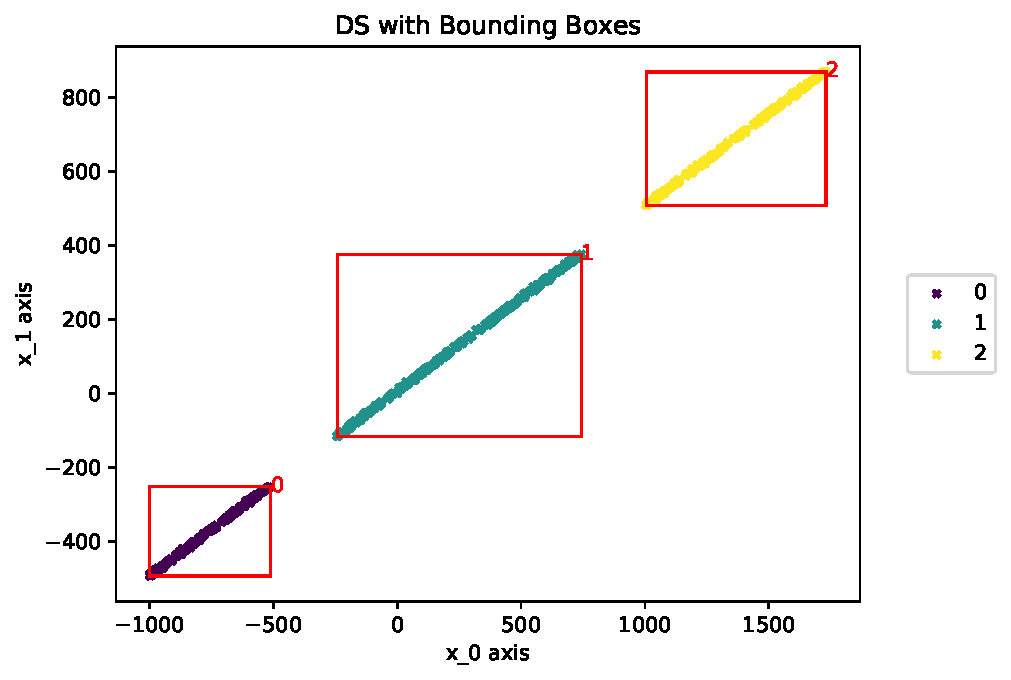
\includegraphics[width=.8\textwidth]{figures/DSwithDBSCANBoundingBoxes.pdf}
      \captionof{figure}{A figure}
      \label{fig:test1}
    \end{minipage}%
    \begin{minipage}{.53 \textwidth}
      \centering
      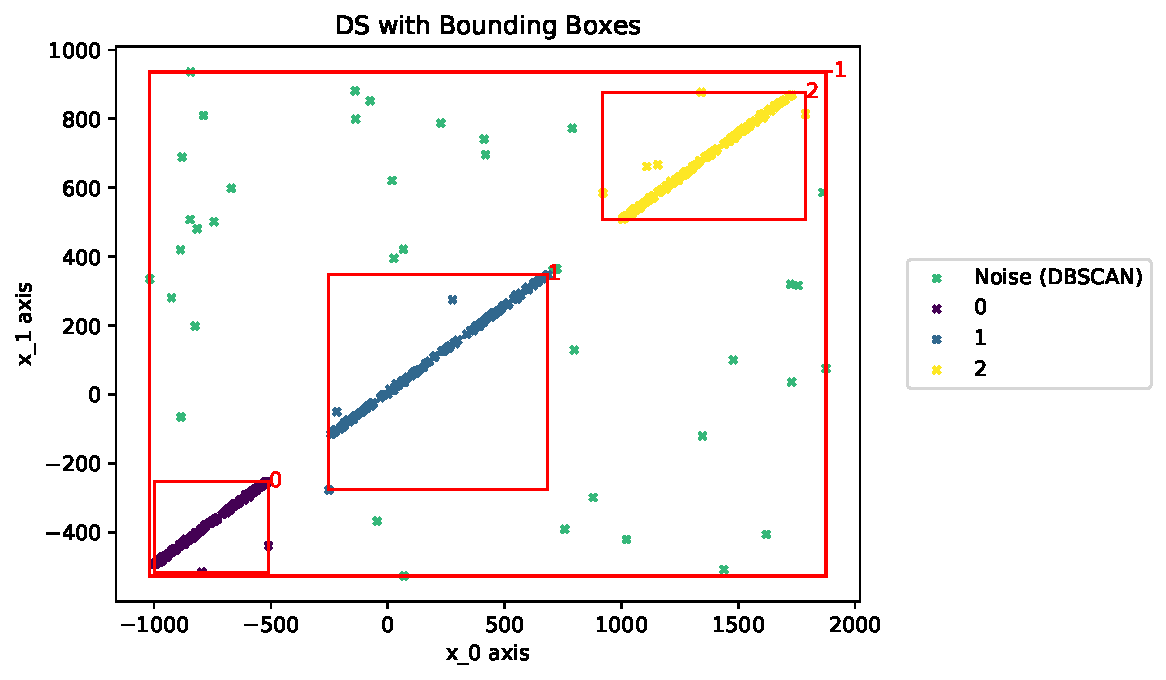
\includegraphics[width=.8\textwidth]{figures/DBSCANwithNoise.pdf}
      \captionof{figure}{Another figure}
      \label{fig:test2}
    \end{minipage}
\end{figure}
To begin with we voted for the use of \gls{dbscan} to retrieve the dense intervals of the original data set. 
As mentioned before the algorithm \gls{dbscan} is categorized into the density-based approach of clustering. This means, that it considers a set of points connected through low proximity in a restricted area/space into similar clusters and thus can, in contrast to partitioning based approaches, create clusters of arbitrary shape (cf. \autoref{fig:kmeansdbscan}). Hence these clusters also can retain information more accurate information about the correlation of the data. Additionally it also directly eliminates noise and can therefore lower the computational cost of the future steps. Its basic principle is as follows:
A group of points is considered as a dense cluster when for each point of the cluster there are sufficiently other points in its neighborhood~\cite{DBSCANEKSX96}.

To understand, how this algorithm works we first have to introduce some terminology.
Given a data set $DS$ of data objects $o$ with a dimensionality of $N$, a distance measure $dist(p_1,p_2))$ and two new parameters, the Epsilon distance $\epsilon$ and the minimum number of points to be a cluster $MinPts$, \citeauthor{DBSCANEKSX96} defines:

\subsubsection*{$\epsilon$-Neighborhood}
% \begin{defn}
The $\epsilon$-Neighborhood $N_{\epsilon}(p)$ of a point $p$ is defined by the set of points $q$ which have a smaller distance $dist(p,q)$ than the threshold $\epsilon$. Formally: 
% \[N_{\epsilon}(p)=\{q \in DS \mid dist(p,q) \leq \epsilon\}\]
\begin{align}
    N_{\epsilon}(p)=\{q \in DS \mid dist(p,q) \leq \epsilon\}
\end{align}

This measure alone however is not enough to fully cluster dense groups, since it would only register points inside the cluster (core points) and omit those at the border of the clusters (border points), since they have less points in their neighborhood. To include those border points too, \citeauthor{DBSCANEKSX96} introduce three more properties/relationships between points.
% \end{defn}

\subsubsection*{(Direct) Density-Reachability}
The direct density-reachability of a point $p$ from another point $q$ is fulfilled if:
% \begin{enumerate}
%     \item $p \in N_{\epsilon}(q)$
%     \item \label{eq:minptsreq}\(|N_{\epsilon}(q)|\geq MinPts\)
% \end{enumerate}
% \begin{flalign}
%     &p \in N_{\epsilon}(q)\label{eq:pinN}&\\\vspace{2mm}
%     &|N_{\epsilon}(q)|\geq MinPts\label{eq:minptsreq}&
% \end{flalign}
\begin{align}
    p \in N_{\epsilon}(q)\label{eq:pinN}\\
    |N_{\epsilon}(q)|\geq MinPts\label{eq:minptsreq}
\end{align}
where \autoref{eq:minptsreq} represents the condition for point \(q\) to be a core point. If a point \(p\) is in the $\epsilon$-Neighborhood of a core point $q$, but itself is not a core point, then point $p$ is labeled as a border point. 

\todor{original sounds way better}
A target point $p$ is density-reachable from origin point $q$, if there is a sequence of connecting points $p, c_1, \dotsc, c_n, q$ in between $p$ and $q$ which are directly density-reachable to its predecessor, e.g. $c_1$ is directly density-reachable from point $q$, $c_2$ is directly density-reachable from point $c_1$, \dots\todor{format} until $p$ is directly density-reachable from point $c_n$. This relation is obviously transitive, but only symmetric if both points of the relation are core points. In case of a border point as the origin there are not enough points in its neighborhood and therefore it does not have any density-reachable neighbor as a target to start with.

\todog{own fig}
\begin{figure}
    \centering
    \begin{minipage}[t]{.5\textwidth}
      \centering  
      \captionsetup{width=.9\linewidth}
      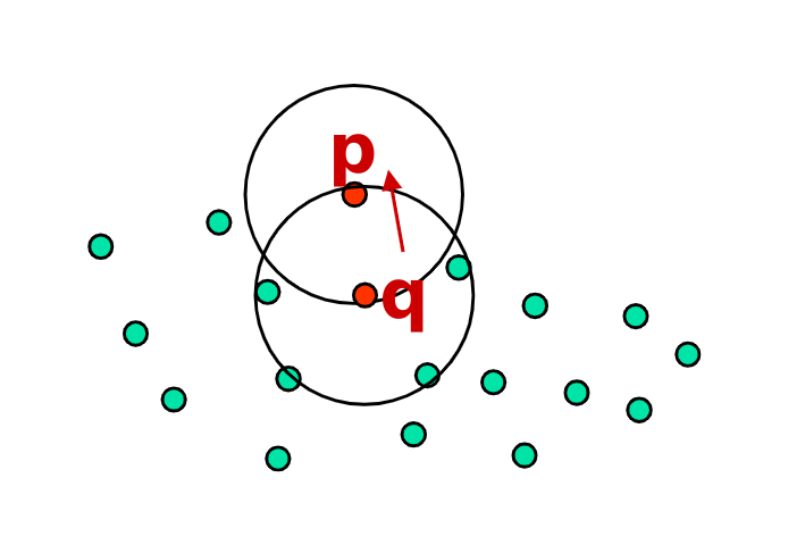
\includegraphics[width=.8\textwidth]{figures/directlydensityreachable.png}
      \captionof*{figure}{Border point p is directly density-reachable from core point q}
      \label{fig:test1}
    \end{minipage}%
    \begin{minipage}[t]{.5\textwidth}
      \centering
      \captionsetup{width=.9\linewidth}
      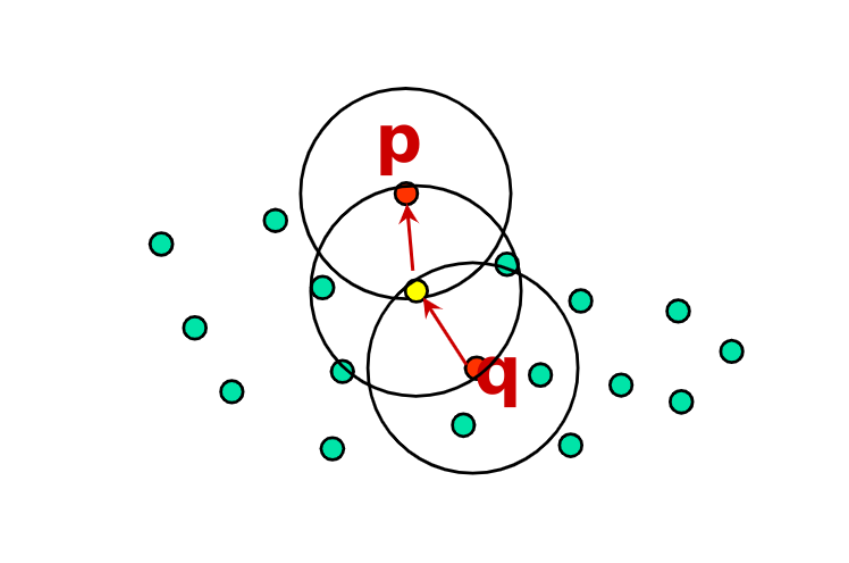
\includegraphics[width=.8\textwidth]{figures/density-reachable.png}
      \captionof*{figure}{p is not directly density-reachable, but density-reachable from q}
      \label{fig:test2}
    \end{minipage}
    \caption{Illustration of reachabilities wrt. $\epsilon$ and $MinPts = 3$, src: KDD-VL}
\end{figure}

\subsubsection*{Density-Connectedness}
The last relation between points is the density-connectedness. Two points $p$ and $q$ are density-connected, if there exists a point $c$, where both points $p$ and $q$ are density-reachable from point $c$. In contrast to the (direct) density-reachability, this relation is symmetric and even reflexive if both points $p$ and $q$ are density-reachable from each other. \todo{generate wider figure saving some space}
\begin{figure}
    \centering
    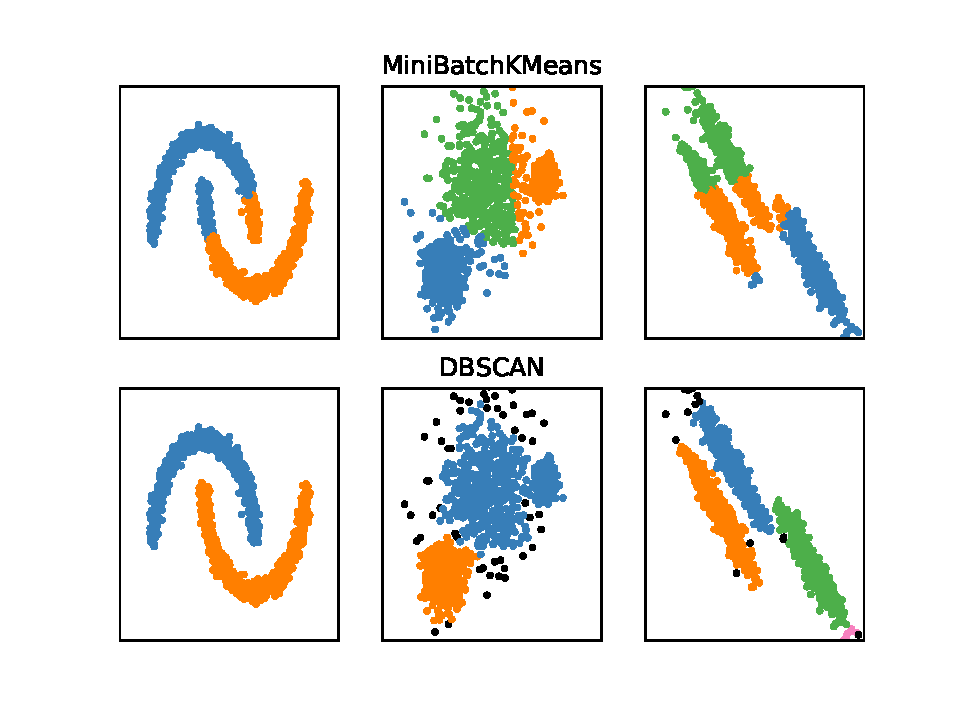
\includegraphics[width=0.7\textwidth]{figures/KMeansVSDBSCAN.pdf}
    \caption{Caption}
    \label{fig:kmeansdbscan}
\end{figure}

\vspace{5mm}

Given the previous defined relations we can now define the notion of clusters and noise in \gls{dbscan}:

\subsubsection*{Density-based Clusters}
A dense cluster is the union of a set of density-connected core points $CP$ and the set of border points $BP$ which are density-reachable from $CP$.
Formally \citeauthor{DBSCANEKSX96} defines a \gls{dbscan}-cluster as:

A dense cluster in data set $DS$ is a non-empty subset $C^{DB} \subseteq DS$ of points $p$ and $q$ if the following two conditions are fulfilled:
\todor{verbatim definition!}
% \begin{enumerate}
%     \item $\forall p, q$: if $p \in C$ and $q$ is density-reachable from $p$, then $q \in C$ (Maximality)
%     \item $\forall p, q \in C$: $p$ is density-connected to $q$ (Connectivity)
% \end{enumerate}
\begin{align}
    &\forall p, q: \text{if } p \in C^{DB} \text{ and } q \text{ is density-reachable from } p \text{, then } q \in C^{DB} \\
    &\forall p, q \in C^{DB}: p \text{ is density-connected to }q
\end{align}

This definition of clustering therefore defines any cluster with \textit{at least} a density defined by the Epsilon-distance $\epsilon$ and the number of minimum points $MinPts$.

\subsubsection*{Density-based Noise}
Every point not belonging to any of the existing clusters $C^{DB}_1, \dotsc, C^{DB}_k$ in data set $DS$ are now considered as noise: 
\begin{align}
    noise^{DB} = \{p \in  DS | \forall i : p \notin C^{DB}_i\}
\end{align}
\todob{transition?}

\subsubsection*{The DBSCAN-Algorithm}
One way to calculate the clusters using \gls{dbscan} is as follows:

First select the first point $p$ of data set $DS$ and check its $\epsilon$-neighborhood. Save every neighbor into a seed list/queue $L$ for further evaluation and check if the neighborhood $N_{\epsilon}(p)$ has enough points to satisfy the $MinPts$-property. 
If it satisfies the property, then point $p$ is a core point and creates a new dense cluster. As long as the seed list is not empty every next point in the list is then classified as either part of the current cluster or noise.
However if $N_{\epsilon}(p)$ does not satisfy the $MinPts$-property, then point $p$ is prematurely labeled as noise. This status will be changed, if another point $q$ has $p$ in its $\epsilon$-neighborhood and itself is a core point, then it is relabeled as a border point of the current cluster.

Then the next point from the seed list $L$ is selected and the same procedure is applied again.
If the seed list $L$ is empty the current cluster is done and the next not previously observed point from $DS$ is evaluated and the whole cycle repeats again until there is no point in the data set $DS$ left.

\vspace{5mm}
\begin{algorithm}[H]
% \algsetup{linenosize=\tiny}
% \scriptsize
\SetAlgoLined
% \DontPrintSemicolon
\KwData{data set $DS$; seed list $L$; current Cluster $C^{DB}_i$; Noise $N^{DB}$; $MinPts$; $\epsilon$}
\KwResult{A set $R$ of clusters $C^{DB}_1,\dotsc,C^{DB}_n$ and noise $N^{DB}$}
 o := first Point of $DS\setminus \{R \cup N\}$\;
 L := [o]\;
 i := 0\;
 \While{$DS\setminus \{R \cup N\}$ is not empty}{
    \While{L is not empty}{
        currentPoint := L.pop(0)\;
        L.push($N_{\epsilon}(currentPoint)$)\;
        \eIf{$|N_{\epsilon}(currentPoint)| > MinPts$}{
            $C^{DB}_i$.add(currentPoint)\;
            $C^{DB}_i$.addAllNeighbors($N_{\epsilon}(currentPoint)$)\;
            N.removeAllNeighbors($N_{\epsilon}(currentPoint)$)\;
        }{
            N.add(currentPoint)
        }
    }
    R.add($C^{DB}_i$)\;
    o := first Point of $DS\setminus \{R \cup N\}$\;
    L := [o]\;
    i := i + 1\;
 }
 \caption{DBSCAN}
\end{algorithm}
\vspace{5mm}

This algorithm was the first approach to segmenting the original data space into subintervals of importance. However, there is a drawback with using \gls{dbscan} as the first segmentation. \gls{dbscan} relies on a global parameter setting which can only find clusters with approximately the same density or higher (c.f. \autoref{fig:DBSCANhierarchy}) and therefore would not be able to find the intrinsic clustering structure well if the underlying models of the global correlations created linear correlations with different densities. 

\begin{figure}
    \centering
    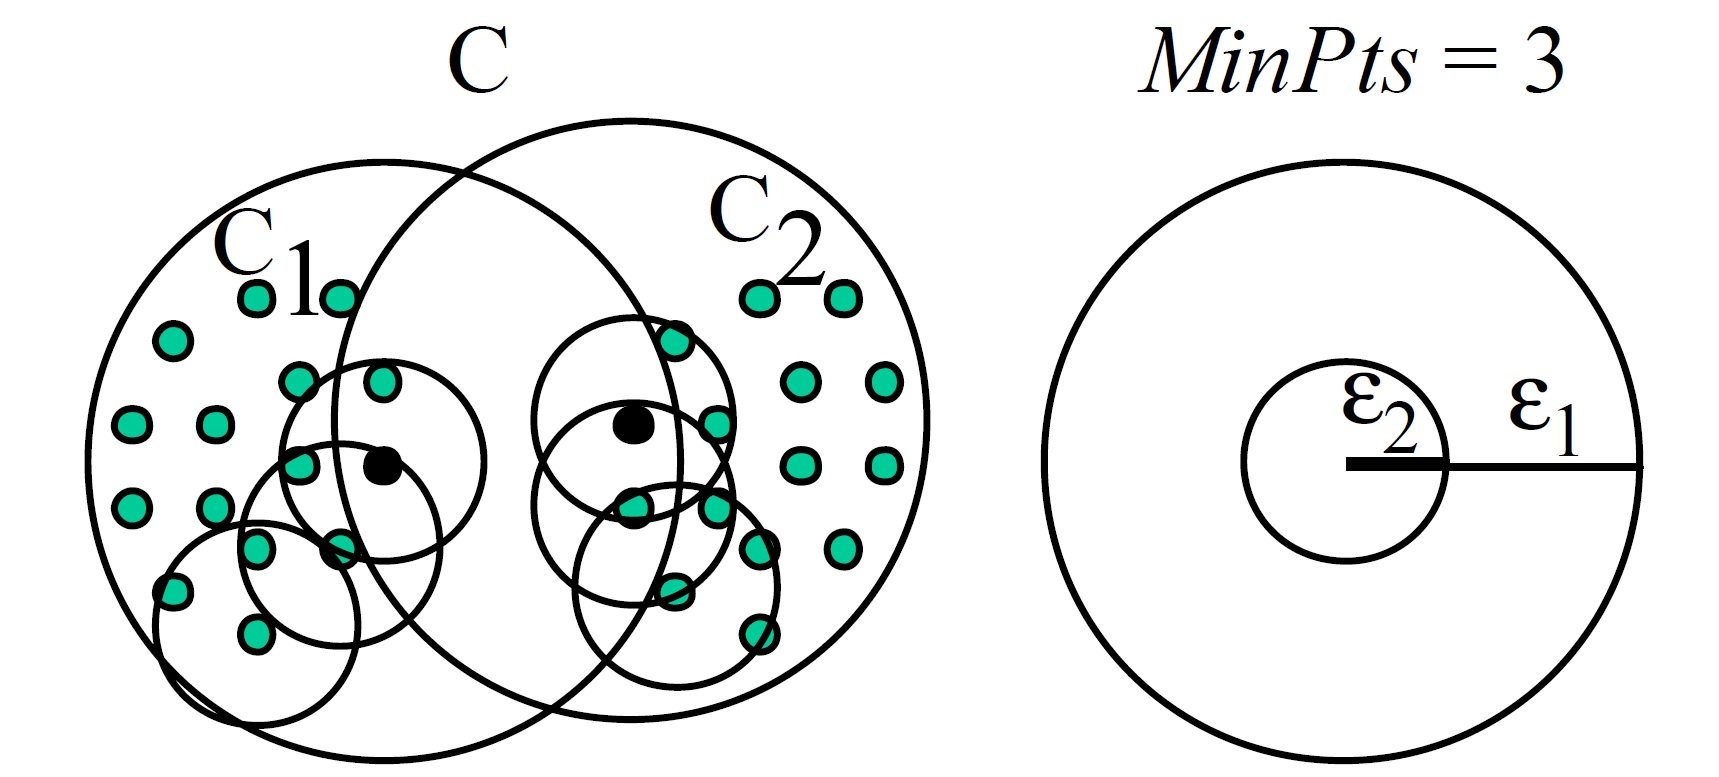
\includegraphics[width=.5\textwidth]{figures/DBSCANleastdensity.png}
    \caption{Caption ~\cite{opticsankerst1999optics}}
    \label{fig:DBSCANhierarchy}
\end{figure}

\subsection{OPTICS - In Depth}\label{ssec:OPTICSindepth} \todob{check comment}%OPTICS ONLY wide range of epsranges, not different minpts, since reachability is dependent on minpts, it extends epsilon, if minpts is not satisfied
To tackle the detection of different densities, we replaced \gls{dbscan} with a more versatile algorithm/extension called \textit{\acrfull{optics}}, which had the capabilities to not only detect clusters of varying densities more accurately, but also opens more possibilities for different further approaches for future work, e.g. a more extensive (bottom-up/hierarchical) approach by evaluating more density-settings at once based on different $\epsilon$-ranges.
Although \gls{optics} itself is not a clustering algorithm, it does create an ordering of the points in a database, which represents the density-based clustering structure of a wide range of $\epsilon$-parameter settings, with which it is possible to automatically create a more accurate clustering with different densities compared to \gls{dbscan}~\cite{opticsankerst1999optics}. To create such a consistent ordering \todo{cite style} \citeauthor{opticsankerst1999optics} defines the following two distances on top of the previously mentioned definitions of \autoref{ssec:DBSCANindepth}:
\vspace{5mm}

Given a point $p$ from the data set $DS$, an epsilon-distance $\epsilon$, the \todor{format} $\epsilon$-neighborhood of $p$ $N_{\epsilon}(p)$, the minimum number of points to be a cluster $MinPts$ and the distance measure from $p$ to its $MinPts$-nearest neighbors $MinPts$-$dist(p)$. Then:
\todo{DBSCAN with one whole cluster instead of 2 separate}
\todor{Figure without bounding box}
\begin{figure}
    \centering
    \begin{minipage}{.47\textwidth}
      \centering
      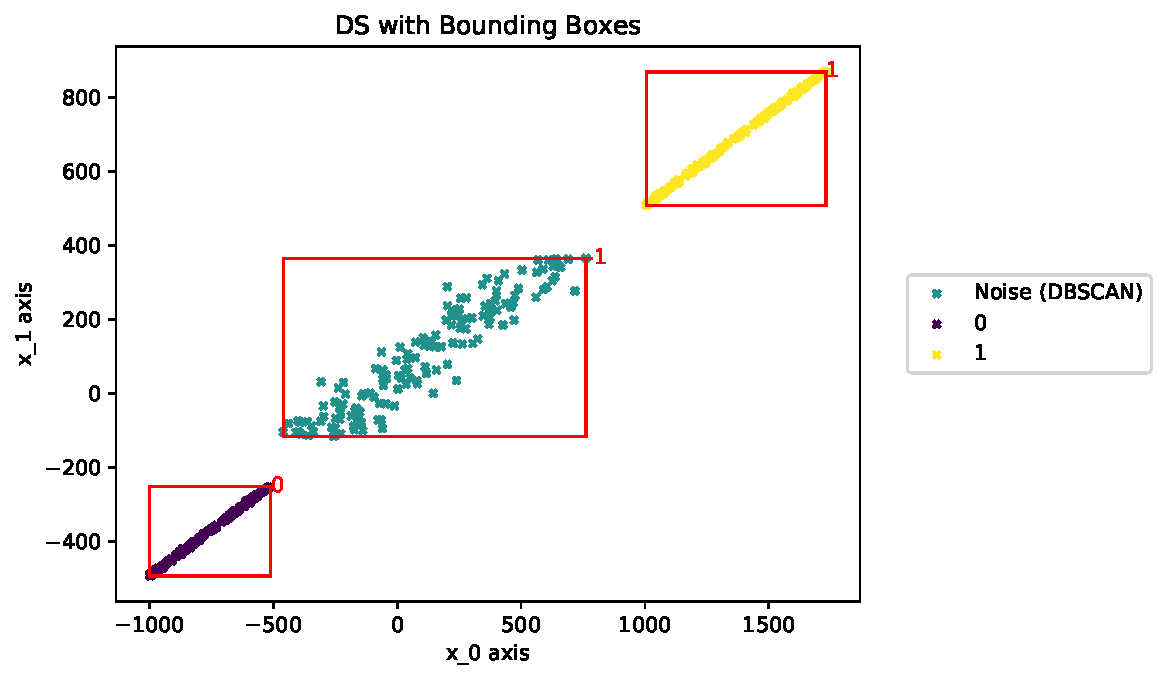
\includegraphics[width=.8\textwidth]{figures/DSwithDBSCANbadBoundingBoxes.pdf}
      \captionof{figure}{A figure}
      \label{fig:baddbscan}
    \end{minipage}%
    \begin{minipage}{.53 \textwidth}
      \centering
      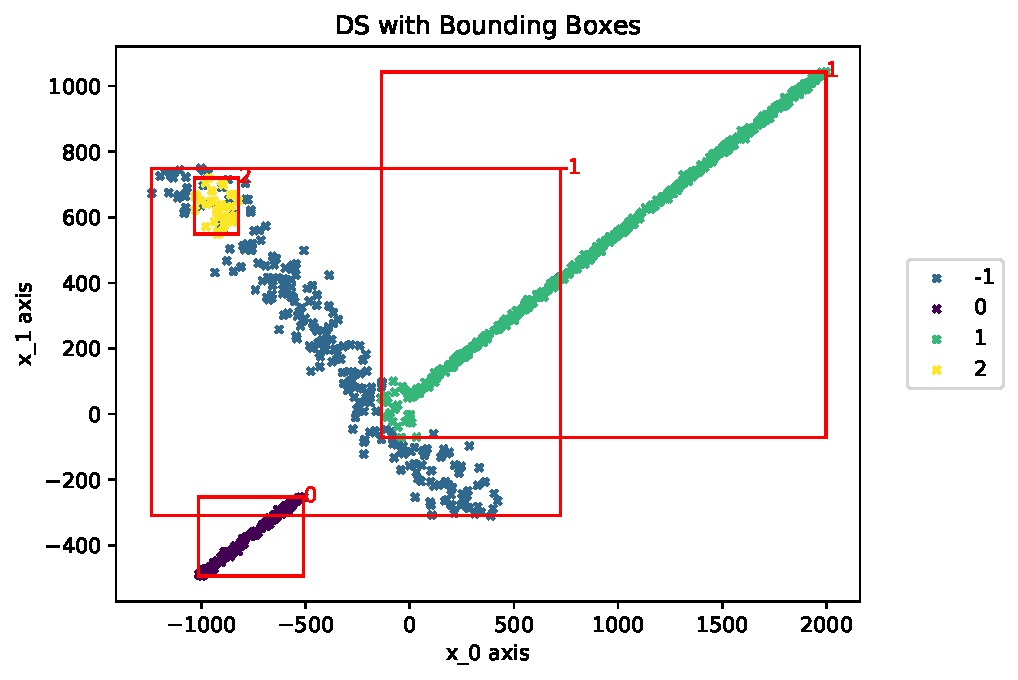
\includegraphics[width=.8\textwidth]{figures/DSwithOPTICSBoundingBoxes.pdf}
      \captionof{figure}{Another figure}
      \label{fig:goodoptics}
    \end{minipage}
\end{figure}

\subsubsection*{Core-Distance}
The core-distance of p describes the smallest  distance $\epsilon_{core}$ with an upper bound of $\epsilon$ such that the number of points in $N_{\epsilon_{core}}(p)$ is greater than $MinPts$, i.e.\ $\epsilon_{core}$ is the smallest epsilon-distance possible for $p$ to be a core point w.r.t.\ to $\epsilon$ and $MinPts$. If $\epsilon_{core}$ exceeds $\epsilon$, then the core-distance of $p$ is \textit{undefined}. Formally the core-distance of p is defined as:
\begin{align}
    core\text{-}dist_{\epsilon,MinPts}(p)=
    \begin{cases}
        \text{undefined} &\text{if } |N_\epsilon(p)| < MinPts\\
        MinPts\text{-}dist(p) &\text{otherwise}
    \end{cases}
\end{align}

\subsubsection*{Reachability-Distance}
The reachability-distance of point $p$ w.r.t.\ another point $q$ is the smallest possible $\epsilon_{reach}$-distance with a lower bound of $core-dist(q)$ such that p is directly-density reachable from q. If $core-dist(q)$ is \textit{undefined}, then $q$ is not a possible core point and the $reach-dist(p,q)$ is also \textit{undefined}. F
Formally the reachability-distance of $p$ w.r.t.\ $q$ is defined as:
\begin{align}
    reach\text{-}dist_{\epsilon,MinPts}(p,q)=
    \begin{cases}
        \text{undefined} &\text{if } |N_\epsilon(q)| < MinPts\\
        max(core\text{-}dist(q), dist(p,q) &\text{otherwise})
    \end{cases}
\end{align}

\subsubsection*{The OPTICS-Algorithm} %This first processed point sound weird
The \gls{optics}-algorithm maintains two data structures to create the ordering, one seed list $L$, which contains (point, reach-dist)-tuples and is ordered by the reach-dist, and the cluster ordering list $O$. 
To create this ordering, \gls{optics} first initializes the ordering $O$ with a random point $o_{proc}$ of $DS$ and a reach-dist of $\infty$. A reachability-distance of $\infty$ from point $a$ w.r.t.\ point $b$ describes that $a$  is simply not contained in the $\epsilon$-neighborhood of $b$ and therefore connected to the dense cluster. Since $o_{proc}$ is the first point of the ordering it does not have a previous cluster to connect to and will never be in the reachability-distance of another point in the ordering. This first point in processing $o_{proc}$ now populates the ordered seed list $L$ with points $o_i$, belonging to the $\epsilon$-neighborhood $N_\epsilon(o_{proc})$, and its reachability-distance w.r.t.\ $o_{proc}$, i.e.\ $reach$-$dist(o_i, o_{proc})$. The further iterations now depend on the state of the seed list $L$. Whenever $L$ is not empty, each next point $o_{proc}$ chosen for processing is taken from the ordered seed list and inserted into the cluster ordering list $O$ with its respective reachability-distance. If $L$ is empty, there is no candidate left to be density-connected and a new $o_{proc}$ is randomly chosen from $DS$ and inserted into $O$ with a reachability-distance of $\infty$ again. The point in process $o_{proc}$ is then used again to populate the seed list. This loop continues until there are no unprocessed points in $DS$ left.

\vspace{5mm}

\begin{algorithm}[H]
% \algsetup{linenosize=\tiny}
% \scriptsize
\SetAlgoLined
\KwData{data set $DS$; seed list $L$ ordered by reach-dist(); cluster order $O$; min \# of pts for a cluster $MinPts$; Eps-distance $\epsilon$}
\KwResult{Ordering $O$ representing the density-based clustering structure}
 L := $\emptyset$\;
 \While{$DS\setminus \{L \cup O\}$ is not empty}{
    \eIf{$L$ is empty}{
        o := random Point of $DS\setminus \{L \cup O\}$\;
        $reach$-$dist$ := $\infty$\;
        $O$.append((o,$reach$-$dist$))\;
    }{
        (o, $saved\ reach$-$dist)$) := $L$.pop(0)\;
        $O$.append((o, $reach$-$dist(o)$))
    }
    \ForEach{$p \in N_\epsilon(o) \setminus \{$O$\}$}{
        $L$.update(($p$, $reach$-$dist(p, o)$))\;
    }
 }
 \caption{OPTICS}
\end{algorithm}
\vspace{5mm}
\todob{maybe chapter about reachability plots}

\subsection{Hough Transformation - In Depth}\label{ssec:houghindepth}
The initial purpose of the Hough transform was a technique to detect colinear points~\cite{houghOriginal1962method} and has since then found various other applications in fields like image processing/analysis~\cite{rosenfeld1969picture,ballard1981generalizing}, computer vision~\cite{davies2004machine} and correlation clustering~\cite{CASHachtert2008robust}.
% \subsubsection{The basic idea}
The basic idea was the transformation of 2-dimensional points $p_i = (x_i,y_i)$ in data space $\mathcal{D} \subseteq \R^2$ with x and y axis to functions in the form of ${m_{p_i}(t_{p_i}) = \frac{y_i}{x_i} - \frac{t_{p_i}}{x_i}}$ in parameter space $\mathcal{P} \subseteq \R^2$, also known as Hough space, with t and m axis, where $m$ is the slope and $t$ is the y-intercept of a line passing through point $p_i$~\cite{illingworth1988survey}. It can be visualized by imagining that each point $p_i$ can be explained by an infinite number of concurrent lines $C$ defined by the functions 
\begin{align}
    {y_{p_i}(m,x) = m \cdot (x - x_i) + y_i}
\end{align}

If we only consider the value of $x=0$ we can still uniquely characterize each equation and instead of the y-value $y_{p_i}$ get the y-intersect $t$ w.r.t.\ slope $m$:
\begin{align}\label{eq:houghparamspace}
\begin{split}
y_{p_i}(m,0) 
&= m \cdot (0 - x_i) + y_i\\
&= -x_i \cdot m + y_i = t(m)
\end{split}\\
\label{eq:hougheq}
\Rightarrow m_{p_i}(t_{p_i}) &= \frac{y_i}{x_i} - \frac{t_{p_i}}{x_i}
\end{align}

A point $p_i = (x_i, y_i)$ in data space is then characterized by each possible $(m,t)$-setting of \autoref{eq:houghparamspace}. In parameter space these continuous $(m_{p_i},t_{p_i})$-settings are uniquely defined by the function in \autoref{eq:hougheq}. A point in data space therefore can be represented as a line in the $(m,t)$-parameter space (c.f.\ \autoref{fig:houghmxt}). \todob{graphing tool} %https://www.yworks.com/products/yed.

\begin{figure}
    \centering
    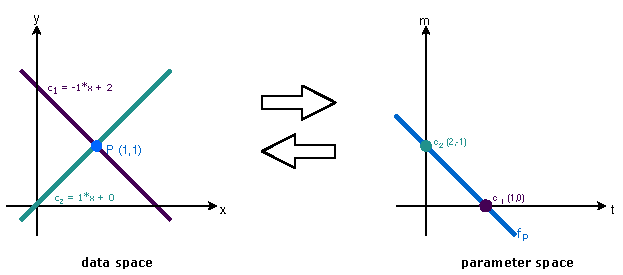
\includegraphics{figures/HoughMXT.pdf}
    \caption{Caption}
    \label{fig:houghmxt}
\end{figure}

However using the slope-intercept form $y = m \cdot x + t$ comes with a drawback, it can not show lines parallel to the y-axis. As a solution \citeauthor{duda1971use} propose the use of the \gls{hnf} for the concurrent lines instead. Their equations in data space change to the following form:
\begin{align}\label{eq:hnfangles}
    \begin{split}
        \delta_{p_i}(\theta_{p_i}) &= x_i \cos{\theta_{p_i}} + y_i \sin{\theta_{p_i}}\\
        &= f_{p_i}(\theta_{p_i})
    \end{split}
\end{align}

where $\delta$ denotes the shortest distance from the respective line to the origin and $\theta$ its respective angle. The parameter space therefore changes to a \mbox{$(\theta,\delta)$-parameter space} and points in data space are transformed to sinusoidal curves instead \todog{own fig}~\autoref{fig:TODOHOUGH}. Since the settings $(\theta,\delta)$ and $(\theta+k\pi,-2\delta)$ represent the same line, $\theta$ is restricted to the interval $[0,\pi)$. Given a point $p_i$ and all angles $\theta_{i,j}$, the distances $\delta_{i,j}$ can be calculated with \autoref{eq:hnfangles}. Hence the parameter space $\mathcal{P}$ can be bounded by $\mathcal{P} = [\delta_{min}, \delta_{max}]\times [0,\pi)$ where $\delta_{min}$ represents the global minimum and $\delta_{max}$ represents the global maximum of all functions $f$ w.r.t. all points. For easier illustration the angle $\theta$ can be transformed into a unit normal vector $\vec{n_0}$ (c.f.\ \autoref{eq:hnfunv}). \todo{hnf fig with $(\theta,\delta)$ and $(\vec{n},\delta)$}

\begin{align}
    \delta &= x_i \cos{\theta} + y_i \sin{\theta}\nonumber\\
    \text{substit}&\text{ute:}\ n_x = \cos{\theta},\ n_y = \sin{\theta} \nonumber\\
    \delta &= x_i n_x + y_i n_y\nonumber\\
    \label{eq:hnfunv}
    \delta &= \vec{n_0}\cdot\vec{x} 
\end{align}

\begin{figure}
    \centering
    % \includegraphics{}
    \missingfigure{hnf visualizations in 2d}
    \caption{Caption}
    \label{fig:my_label}
\end{figure}

\begin{figure}
    \centering
    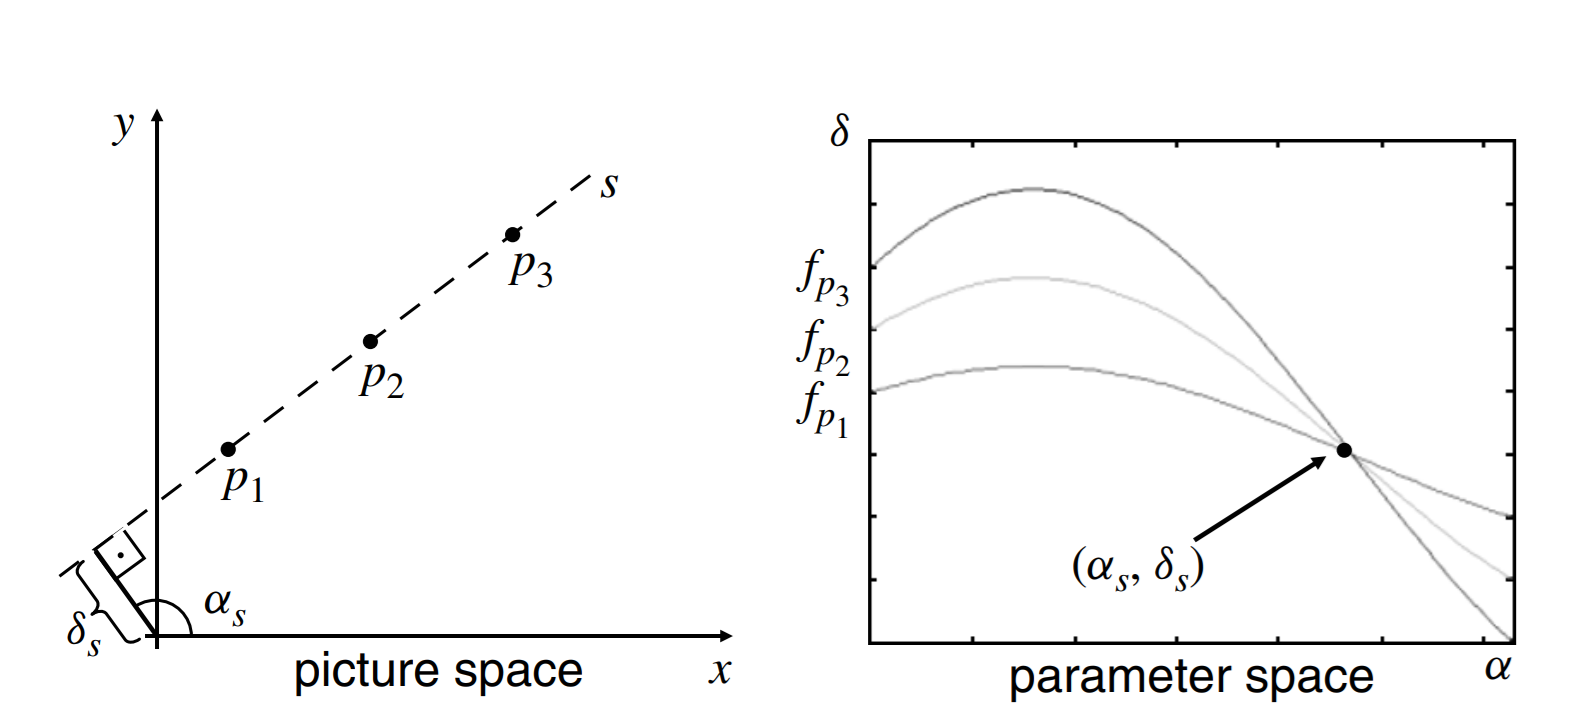
\includegraphics[width=0.7\textwidth]{figures/TODOHOUGHTHETADIST.png}
    \caption{\cite{CASHachtert2008global}}
    \label{fig:TODOHOUGH}
\end{figure}

Summarized this duality between data and parameter space results in the following properties:\label{ssec:properties}
\todor{choose a style}
\begin{property}\label{prop:hough1}
A point in data space corresponds to a (sinusoidal) function in the parameter space. 
\end{property}
\begin{property}\label{prop:hough2}
A point in parameter space corresponds to a linear function in the data space.
\end{property}
\begin{property}\label{prop:hough3}
Points lying on the same line in data space have a common intersection in parameter space.
\end{property}
\begin{property}\label{prop:hough4}
Points lying on the same (sinusoidal) function in parameter space correspond to lines through the same point in data space.
\end{property}

Since points in parameter space correspond to a linear function in data space and a curve in parameter space corresponds to a point in data space, we can deduct that intersections of curves in parameter space correspond to points lying on the same line in data space. Therefore through the transformation the problem of finding correlated points becomes a problem of finding points or regions of intersections of curves in parameter space. Another added benefit is the parameter space's independence of the locality assumption since regardless of the points locations in data space its functions intersections in parameter space represent points lying on the same line. \todor{wtf sentence} To solve this problem there are several approaches. For exact results looking for points with high intersections can be done by solving linear equation systems of the functions in parameter space. This however can quickly become computationally infeasible and does not cope for jitter, which causes disruptions in the exact intersections in parameter space. Static predefined grid-based approaches, like searching for 2-dimensional regions of interest with a predefined grid/accumulator using a voting scheme, or dynamic approaches, like done in \textcite{CASHachtert2008global} by splitting the 2d search space more efficiently, are some computationally less expensive solutions. An in-depth explanation of one approach, namely \acrfull{cash}, will be given in \fullref{ssec:CASHindepth}.

\subsection{CASH - In Depth}\label{ssec:CASHindepth}
\todo{check n-dim Hough transform explanation with DK}
\acrfull{cash} is a subspace clustering algorithm based on the principle of the Hough Transform which, in contrast to the axis-parallel algorithms \acrshort{subclu}\cite{sublcukailing2004density} and \acrshort{clique}\cite{cliqueagrawal1998automatic}, can detect arbitrarily oriented subspaces (c.f.~\autoref{ssec:houghindepth}. \todor{sounds awful}
For arbitrary-dimensional data spaces $\mathcal{D} \subseteq \R^d$ \textcite{CASHachtert2008robust} reformulates the Hough transformation via a generalized description of spherical coordinates. A $d$-dimensional point/vector $x=(x_1,\dotsc,x_d)$ w.r.t.\ the given orthonormal basis $e_1,\dotsc,e_d$, can be described with $d-1$ independent angles $\alpha_1,\dotsc,\alpha_{d-1}$ and the norm/distance to origin of vector/point $x$. The following definitions are taken from \cite{CASHachtert2008robust}:

\subsubsection*{Spherical Coordinates}\label{def:spherecord}
\todor{verbatim definition!}
Let $e_i, 1 \leq i \leq d$, be an orthonormal basis in a $d$-dimensional feature space. Let $x=(x_1,\dotsc,x_d)$ be a $d$-dimensional vector on the hypersphere of radius $r$ with center at the origin. Let $u_i$ be the unit vector in the direction of the projection of $x$ onto the manifold spanned by $e_i,\dotsc,e_d$. For the $d-1$ independent angles $\alpha_1,\dotsc,\alpha_{d-1}$, let $\alpha_i$, $1 \leq i \leq d-1$, be the angle between $u_i$ and $e_i$. Then the generalized spherical coordinates of vector $x$ are defined by:
\begin{align}
    x_i = r \cdot (\prod_{j=1}^{i-1}\sin{\alpha_j}) \cdot \cos{\alpha_i}\text{, where } \alpha_d = 0.
\end{align}

Similar to \autoref{ssec:houghindepth} any $d$-dimensional point $p \in \mathcal{D}$ can be explained by an infinite number of hyperplanes containing $p$. These hyperplanes can be uniquely defined by the $d-1$ angles $\alpha_1,\dotsc,\alpha_{d-1}$, with $\alpha_i \in [0,\pi)$ representing the normal vector of the hyperplanes, and a fix point $o$ on the hyperplane. To acquire a point independent representation \textcite{CASHachtert2008robust} maps the angles $\alpha_i$ and point $p$ with the following parametrization function to the shortest distance $\delta$ of the hyperplane to the origin (c.f. \ref{eq:hnfangles}).

\subsubsection*{Parametrization Function}
Let $\vec{p} = (p_1,\dotsc,p_d)$ be a $d$-dimensional vector and $\vec{n_0} = (n_1,\dotsc,n_d)$ be a $d$-dimensional unit vector specified by $d-1$ angles $\alpha_1,\dotsc,\alpha_{d-1}$ according to the \hyperref[def:spherecord]{previous definition \textit{``Spherical Coordinates''}}. Then the parametrization function $f_{\vec{p}}:\R^{d-1} \rightarrow \R$ of vector $\vec{p}$ denotes the distance of the hyperplane defined by the point $p$ and the normal vector $\vec{n}$ to the origin:
\begin{align}
    \begin{split}
            f_{\vec{p}}(\alpha_1,\dotsc,\alpha_{d-1}) &= \langle \vec{p},\vec{n_0} \rangle\\
    &= \sum_{i=1}^d p_i \cdot (\prod_{j=1}^{i-1} \sin{\alpha_j}) \cdot \cos{\alpha_i}  = \delta
    \end{split}
\end{align}

Given $d-1$ angles $\alpha_1,\dotsc,\alpha_{d-1}$ and shortest distance $\delta$ obtained by the parametrization function for a point $p_i = (x_1,\dotsc,x_d)$ and its infinite hyperplanes, each point $p$ in data space $\mathcal{D}$ can be mapped to a $d$-dimensional parameter space $\mathcal{P} \subseteq \R^d$ spanned by the previously mentioned parameters, again creating a function defining a hyperplane:
\begin{align}
    \begin{split}
        \delta &= x_1 \cdot n_{0,1} + \dots + x_d \cdot n_{0,d}\\
        &= \langle \vec{x},\vec{n_0} \rangle\label{eq:highhnf}
    \end{split}
\end{align}
Similar to \autoref{ssec:houghindepth} the resulting hyperplane in parameter space can be transformed between  cartesian representation using a unit vector $\vec{n_0}$ and polar representation based on angles $\alpha_1,\dotsc,\alpha_{d-1}$. In the process of this thesis, we primarily use the cartesian form of the \gls{hnf} (c.f. \autoref{eq:highhnf}).


By the means of the parametrization function \textcite{CASHachtert2008robust} extend the properties of the original Hough transformation (c.f. \autoref{ssec:properties}) to $d$-dimensional data spaces and its corresponding parameter spaces: \todor{verbatim}
\begin{quoting}
\begin{property}
A point $p$ in data space $\mathcal{D} \subseteq \R^d$ is represented by a sinusoidal curve $f_p:\R^{d-1}\rightarrow\R$ in parameter space.
\end{property}
\begin{property}
A point $p' = (\alpha_1,\dotsc,\alpha_{d-1},\delta$ in parameter space $\mathcal{P} \subseteq R^d$ corresponds to a $(d-1)$-dimensional hyperplane in data space.
\end{property}
\begin{property}
Points that are located on a $(d-1)$-dimensional hyperplane in data space correspond to sinusoidal curves through a common point in parameter space.
\end{property}
\begin{property}
Points lying on the same sinusoidal curve in parameter space represent $(d-1)$-dimensional hyperplanes through the same point in data space.
\end{property}
\end{quoting}

% \begin{enumerate}
%     \item A point $p$ in data space $\mathcal{D} \subseteq \R^d$ is represented by a sinusoidal curve $f_p:\R^{d-1}\rightarrow\R$ in parameter space.
%     \item A point $p' = (\alpha_1,\dotsc,\alpha_{d-1},\delta$ in parameter space $\mathcal{P} \subseteq R^d$ corresponds to a $(d-1)$-dimensional hyperplane in data space.
%     \item Points that are located on a $(d-1)$-dimensional hyperplane in data space correspond to sinusoidal curves through a common point in parameter space.
%     \item Points lying on the same sinusoidal curve in parameter space represent $(d-1)$-dimensional hyperplanes through the same point in data space.
% \end{enumerate}
\missingfigure[]{3d example, fig anfragen}
\begin{figure}
    \centering
    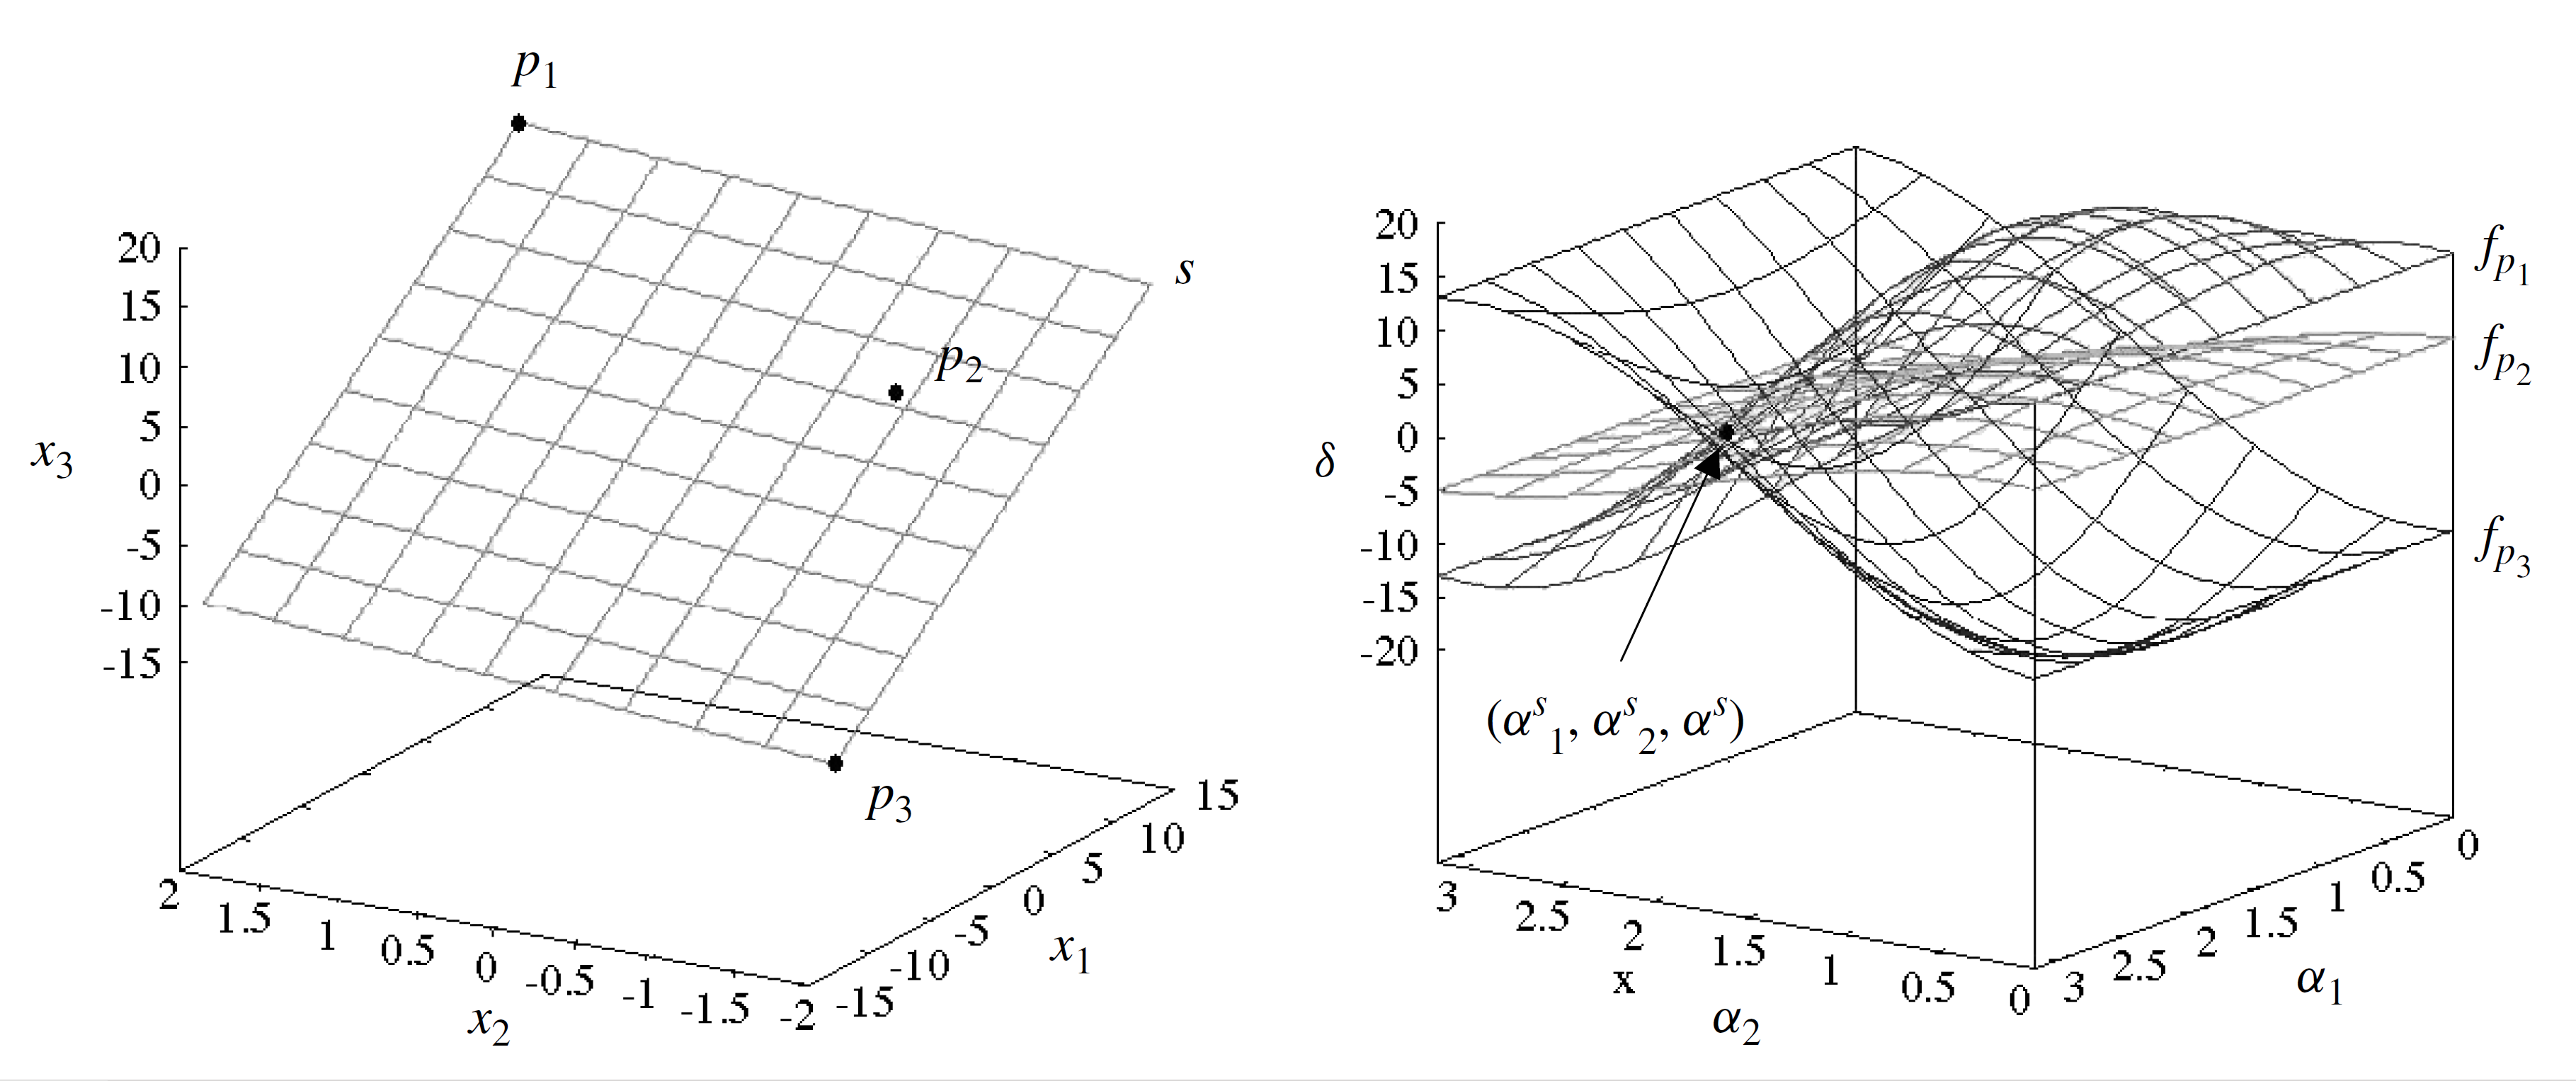
\includegraphics[width=0.9\textwidth]{figures/cash3d.png}
    \caption{Caption}
    \label{fig:my_label}
\end{figure}

Boundaries of the parameter space $\mathcal{P}$ are extended to $\mathcal{P} = [\delta_{min}, \delta_{max}]\times [0,\pi)^{d-1}$ with $\delta_{min}$ and $\delta_{max}$ being the minimum and maximum of all functions $f_p$ for $\alpha \in [0,\pi)$ again: $[\delta_{min}, \delta_{max}] = [min_{p \in \mathcal{D}}(f_p(\alpha_p^{min})), max_{p \in \mathcal{D}}(f_p(\alpha_p^{max}))$, where $\alpha_p^{min}$ and $\alpha_p^{max}$ denote the minimum and maximum of function $f_p$. An in detail explanation is found in \textcite{CASHachtert2008robust}.
Applying the same concept of \autoref{ssec:houghindepth} the goal of finding $d$-dimensional points lying on the same hyperplane requires finding intersections of the corresponding $d$-dimensional curves in parameter space. Since an analytical solution of the intersections in multi-dimensional space is infeasible, the parameter space is scanned for $d$-dimensional regions/hypercuboids of a certain amount $m$ of intersections instead which additionally copes for jitter. Regions which fulfill the number of intersections are called \textit{dense grid cells}.

\subsubsection*{Correlation Cluster}\todor{check definition with dk}
Since we have to distinguish correlation clusters from density-based clusters, we hereby propose a notion of correlation clusters.

Correlation in a classical sense is a measure of relationship between two variables/features, but can also be extended to relations between multiple features. Commonly the relation refers to a linear relationship, but can also be non-linear. Since we want to cluster these correlations not only by orientation, but also by positioning, we define a specifically located correlation $r_{l,f,t}$, with $l$ being an unambiguous location as the source of the correlation, $f$ being a set of predictor features and $t$ being the target/correlating feature, as a hyperplane $h(t,f,l)$. In case of \gls{cash} a localized correlation/hyperplane is defined by the \gls{hnf}(c.f. \autoref{eq:highhnf}) with $f$ and $t$ being embedded in the orientation $n_{0,i} \in \{f,t\}$ and distance $\delta$ and $l$ only being embedded in the latter one. 
\begin{align}
    \delta(t,f,l) = \langle \vec{x},\vec{n_0}(f,t) \rangle
\end{align}
\textit{Correlation clusters} refer to the grouping of observations/data objects within a certain interval in data space which display similar correlations in a subset of the objects features. In other words a Correlation Cluster is a group of points which have a low distance $j$, which we will refer to as \textit{jitter}, to a hyperplane $h$ modeled by a correlation within an interval. We formalize it as following:

A correlation cluster in data set $DS$ is a non-empty subset $C^{Corr} \subseteq DS$ of points $p$ which fullfill the following condition:
\begin{align}
    &\forall p: \text{if } \text{dist}(p,h) < j \text{, then } p \in C^{Corr}
\end{align}

where the function $dist(a,b)$ denotes the shortest distance between two geometric\todor{richtiger begriff dafuer?} objects, $h$ being the hyperplane modeling the localized correlation and $j$ the jitter representing the maximal threshold for fault tolerance.

\todor{eigene definition, consistent with dbscan}

\subsubsection*{Correlation Noise}
Analogous to density-based noise in \autoref{ssec:DBSCANindepth}, every point not belonging to any of the existing clusters $C^{Corr}_1, \dotsc, C^{Corr}_k$ in data set $DS$ are now considered as noise: 
\begin{align}
    noise^{Corr} = \{p \in  DS | \forall i : p \notin C^{Corr}_i\}
\end{align}

\subsubsection*{The CASH-Algorithm}
Given previously defined data representation in data and parameter space, the goal is finding dense grid cells in parameter space. However since the complexity of searching the parameter space with a predefined grid is exponential w.r.t.\ dimension $d$ it also quickly gets too computational expensive for higher dimensional spaces. \gls{cash} tackles this problem by smartly dividing the search space. \citeauthor{CASHachtert2008robust} proposed the following search strategy:
\vspace{5mm}

The parameter space is successively divided by the axes in the static order given by $\delta,\alpha_1,\dotsc,\alpha_{d-1}$. After each split the hypercuboid with more intersections is divided at the next axis of the order. If both hypercuboids have the same amount of intersections, the first hypercuboid is selected (arbitrarily). The other hypercuboid is kept in a queue, which is ordered descendingly by the number of its intersecting curves/points. If regions in the queue have an equal amount of intersections, the smaller region is preferred. These splits and additions to the queue are done until both split hypercuboids have less than a minimum number of intersections $m$ to be considered as dense or a predefined depth $s$ has been reached and the hypercuboids fulfilling $m$ and are dense are considered as valid subspace clusters. These valid $(d-1)$-dimensional subspace clusters are then recursively evaluated by CASH again until the resulting found subspace clusters have a minimum dimensionality of $minDims$. If a subspace cluster is found, its intersecting curves are removed from any other hypercuboid in the queue, which is then updated and sorted according to its new status. If the number of intersections drops below $m$, the hypercuboid is removed from the queue. This procedure is done, until the queue is empty.

\vspace{5mm}
\begin{algorithm}
% \algsetup{linenosize=\tiny}
% \scriptsize
\SetAlgoLined
\KwData{parameter space $\mathcal{P}$; queue $Q$ ordered by number of intersections and its volume; iterator $I$ of order of axis $[\delta,\alpha_1,\dotsc,\alpha_{d-1}]$; set of subspace clusters $C$; minimum number of intersections $m$; maximum number of splits $s$}
\KwResult{Set of clusters $C$ representing the subspaces found in $\PS$}
\SetKwFunction{CASH}{CASH}
\SetKwProg{Fn}{Function}{:}{\KwRet $C$}
Q := $\emptyset$\;     
h1 := first hypercuboid of split\;
h2 := second hypercuboid of split\;
h := $\PS$\tcp*{working hypercuboid}
\Fn{\CASH{$h$, $m$, $s$}}{
     \Do{$Q$ is not empty}{
        h1, h2 := h.splitAxis($I$.next())\;
        h := $arg\,max_{cube \in \{h1,h2\}}(cube.intersections)$\;
        Q.add(\{h1,h2\}$\setminus$ h)\;
        splitcounter := 1\;
        \While{$h.intersections > m$ and $splitcounter < s$}{
            h1, h2 := h.splitAxis($I$.next())\;
            splitcounter++\;
            h := $arg\,max_{cube \in \{h1,h2\}}(cube.intersections)$\;
            Q.add(\{h1,h2\}$\setminus$ h)\;
        }
        \If{$h.intersections > m$}{
            $C := C\ \cup$\ \CASH{h,m,s}\;
        }
        $I$.reset()\tcp*{reset Iterator for split of next $h$}
        $Q$.removeIntersectionsAndUpdate($C$)\;
    }
}

 \caption{CASH}
\end{algorithm}
\vspace{5mm}

The resulting set $C$ contains all $n$-dimensional subspace clusters with $n < d$ found within the constraints of minimum points in correlation $m$ and maximum splits $s$.
\todor{Check recursive CASH}

Summarized we now possess means to find density-based clusters and global subspace clusters in an original data set $DS$. The density-based approach \gls{optics} requires two parameters, minimum number of points $minPts$ and a maximum epsilon distance $\epsilon$, which essentially specify the minimum density allowed, to acquire a hierarchical view of density-connected clusters in $DS$. The subspace clustering approach \gls{cash} also requires another two parameters, minimum number of points/intersections $m$ and number of splits $s$ to be considered as a subspace cluster.

\section{The Algorithm}
With the previously mentioned algorithms we are already able to find arbitrarily shaped clusters with a density-based approach, and arbitrarily oriented subspace clusters with e.g. \gls{4c} or \gls{cash}, however all of them are restricted to finding those clusters in a purely local or purely global fashion. E.g. none of the previously mentioned algorithms can handle scenarios as shown in 
% \begin{minipage}{.47\textwidth}
%       \centering
%       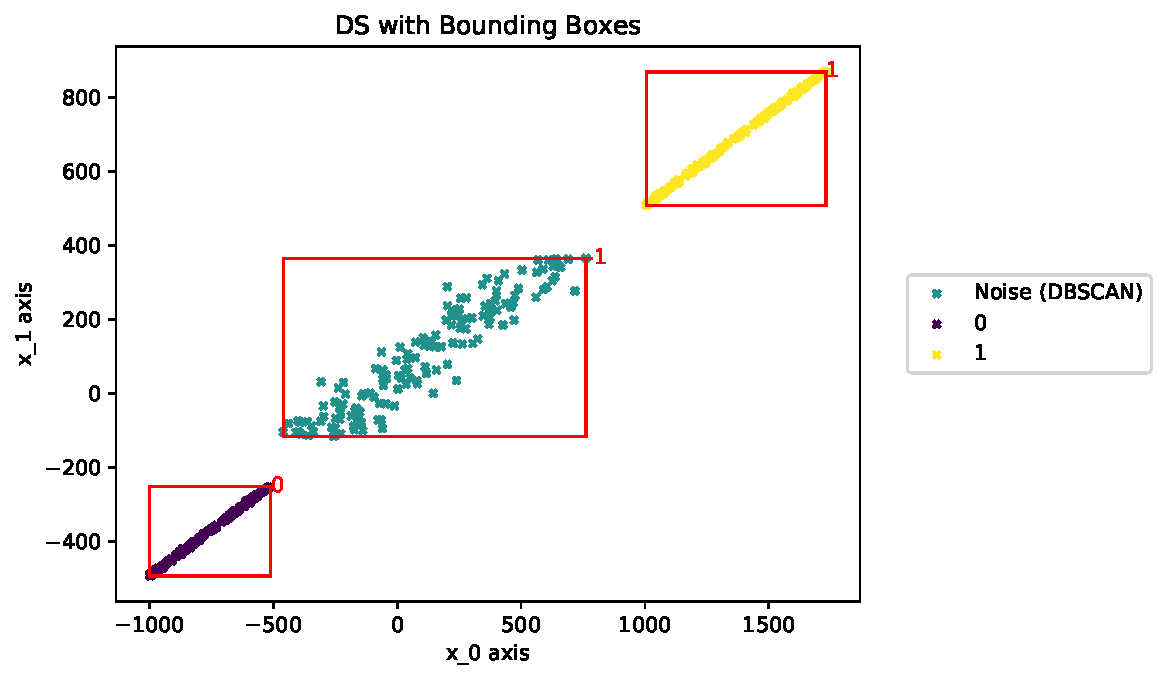
\includegraphics[width=.8\textwidth]{figures/DSwithDBSCANbadBoundingBoxes.pdf}
%       \captionof{figure}{A figure}
%       \label{fig:baddbscan}
%     \end{minipage}%
%     \begin{minipage}{.53 \textwidth}
%       \centering
%       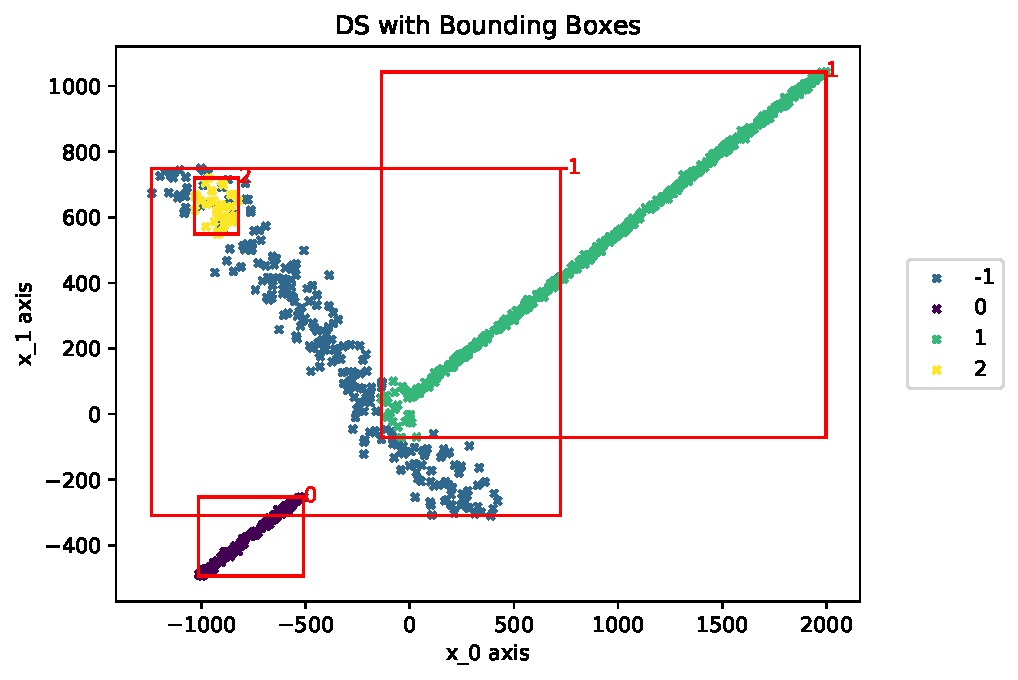
\includegraphics[width=.8\textwidth]{figures/DSwithOPTICSBoundingBoxes.pdf}
%       \captionof{figure}{Another figure}
%       \label{fig:goodoptics}
%     \end{minipage}
\begin{figure}
    \centering
    \includegraphics{}
    \missingfigure[]{scenario zeigen}
    \caption{Caption}
    \label{fig:}
\end{figure}
Above Figures \todor{figure erstellen} depict settings, where the data contains multiple characteristic local correlations which however cannot be accurately described by the aforementioned methods alone. Figure 1 shows cross-shaped dense clusters which can be picked up by \gls{dbscan} or \gls{optics}, however it does not deliver their correlations. As an extension \gls{4c} is able to detect the local correlations, however gets skewed results in the crosses due to the correlations orientation not being accurately representable by the eigenvectors of the \gls{pca}\cite{PCAshlens2014tutorial}. 
\gls{cash} on the other hand could find the correlations. 

\begin{figure}
    \centering
    \includegraphics{}
    \missingfigure[]{local global problem}
    \caption{Caption}
    \label{fig:localglobalproblem}
\end{figure}

\autoref{fig:localglobalproblem} \todor{figure} shows multiple local settings of different correlations. \gls{4c} is able to find the accurate local correlations, however can not categorize those local correlations as one global correlation. 
On the other hand \gls{cash} can only find the global correlation while omitting the information of the gaps in data. Hierarchical subspace clustering methods like \acrshort{hico} and \acrshort{eric} do not address the problem either, since their hierarchy is also based on global lower dimensional subspaces contained in the original space and not spaces composed of same dimensional subintervals of the same space. These subintervals of a space further will be referred as \textit{subclusters} or \textit{clusterpartitions}\todor{2 begriffe oder lieber consistent einen benutzen?}.
So either the subspace clustering method detects local correlations while missing the big picture or they do find global correlations while losing structural information of its particular correlation. This thesis proposes an algorithm that unifies local and global correlation clustering by evaluating \textit{locally dense} regions of interest with a correlation clustering method, e.g. \gls{cash}, and combining those local intermediate correlations into a global correlation clustering to get a universal subspace clustering result. 

%Additionally it does not categorize both horizontal local correlations as one, even though they arguably could be interpreted that way.
% , not the big picture

\subsection{Partitioning Data into Dense Clusters}
The first step we perform is the partitioning of the data space into dense clusters via a density-based clustering approach like \gls{dbscan} or \gls{optics}. 
%However like mentioned in \autoref{ssec:DBSCANindepth} and \autoref{ssec:OPTICSindepth}
Since we want to find \textit{local} linear correlations within \textit{global} linear correlations, we assume that the global linear correlation is composed of a set of its local linear correlations. This also means that points belonging to the same global linear correlation are also part of the composing local subclusters which have a similar inherent linear correlation as the global correlation. These subclusters have a continuous distribution of density compared to the global correlation itself, since else it would have been split as well and counted as separate local subcluster. Vice versa the local components are also disjunct to each other, since else there would be a connection to each other to create a bigger clusterpartition. Although it is not optimal even if there is an overlap of different global linear correlations and the clusterpartition contains multiple of them, it still can retain the information of its composing linear correlations.
We can therefore retrieve these local subclusters by searching the data for density-connected sets of points via a density-based clustering approach like \gls{dbscan} or \gls{optics}. This comes with an additional benefit by automatically removing noise. 

However like mentioned in \autoref{ssec:DBSCANindepth} and \autoref{ssec:OPTICSindepth} \gls{dbscan} is not able to find clusters with different density and mixes multiple densities together into one cluster due to its global parameter setting only defining a minimum density. High variance in data densities can therefore strongly influence the result of \gls{dbscan}, either by making it harder to choose the appropriate parameters for a better clustering result or by having more variety in density in found clusters which would result in less conclusive detection of their linear correlations. 
To receive a more suited clustering we preferred the use of \gls{optics}, which is able to detect clusters with different densities (c.f.~\autoref{ssec:OPTICSindepth}). Since we do not want to prune any information away we can generally use a very high epsilon-distance $\epsilon$ to create a detailed ordering and therefore only rely on $MinPts$ as a parameter. From this ordering we can extract clusters with a new parameter $reachdist_{thres}$ which represents the threshold at which the difference of neighboring reachability-distances of the ordering is considered to be a new cluster with different density. We also assign a bounding box for each found cluster, which represents the local data space for further evaluation performed by \gls{cash}. Up to this point we are merely partitioning the data into dense clusters with the added benefit of filtering out points $noise_{density-based}$ which are considered as noise points by a density-based view. We will reconsider those noise points later, since they still could be parts of the global correlation clustering despite not being dense. Figure x visualizes a data set after step 1 is performed. The relevant part of the data set is clustered by density and its boundaries are highlighted by the bounding boxes.
\missingfigure[]{figure with bounding box}

\subsection{Finding Local Linear Correlations}
Based on the assumption that local linear correlations contained in a global linear correlation have similar orientations as their parents\todor{parent richtiger begriff?}, we extract all correlations of the dense clusters with a subspace clustering method and in a later step combine them and rebuild the global correlation clustering. The second step therefore is the extraction of all local linear correlations of all dense clusters within its respective bounding box in data space. Since we only consider the points of the locally dense subclusters without/less noise we can use a variety of methods to extract the linear correlations via global subspace clustering algorithms. 

\begin{figure}
    \centering
    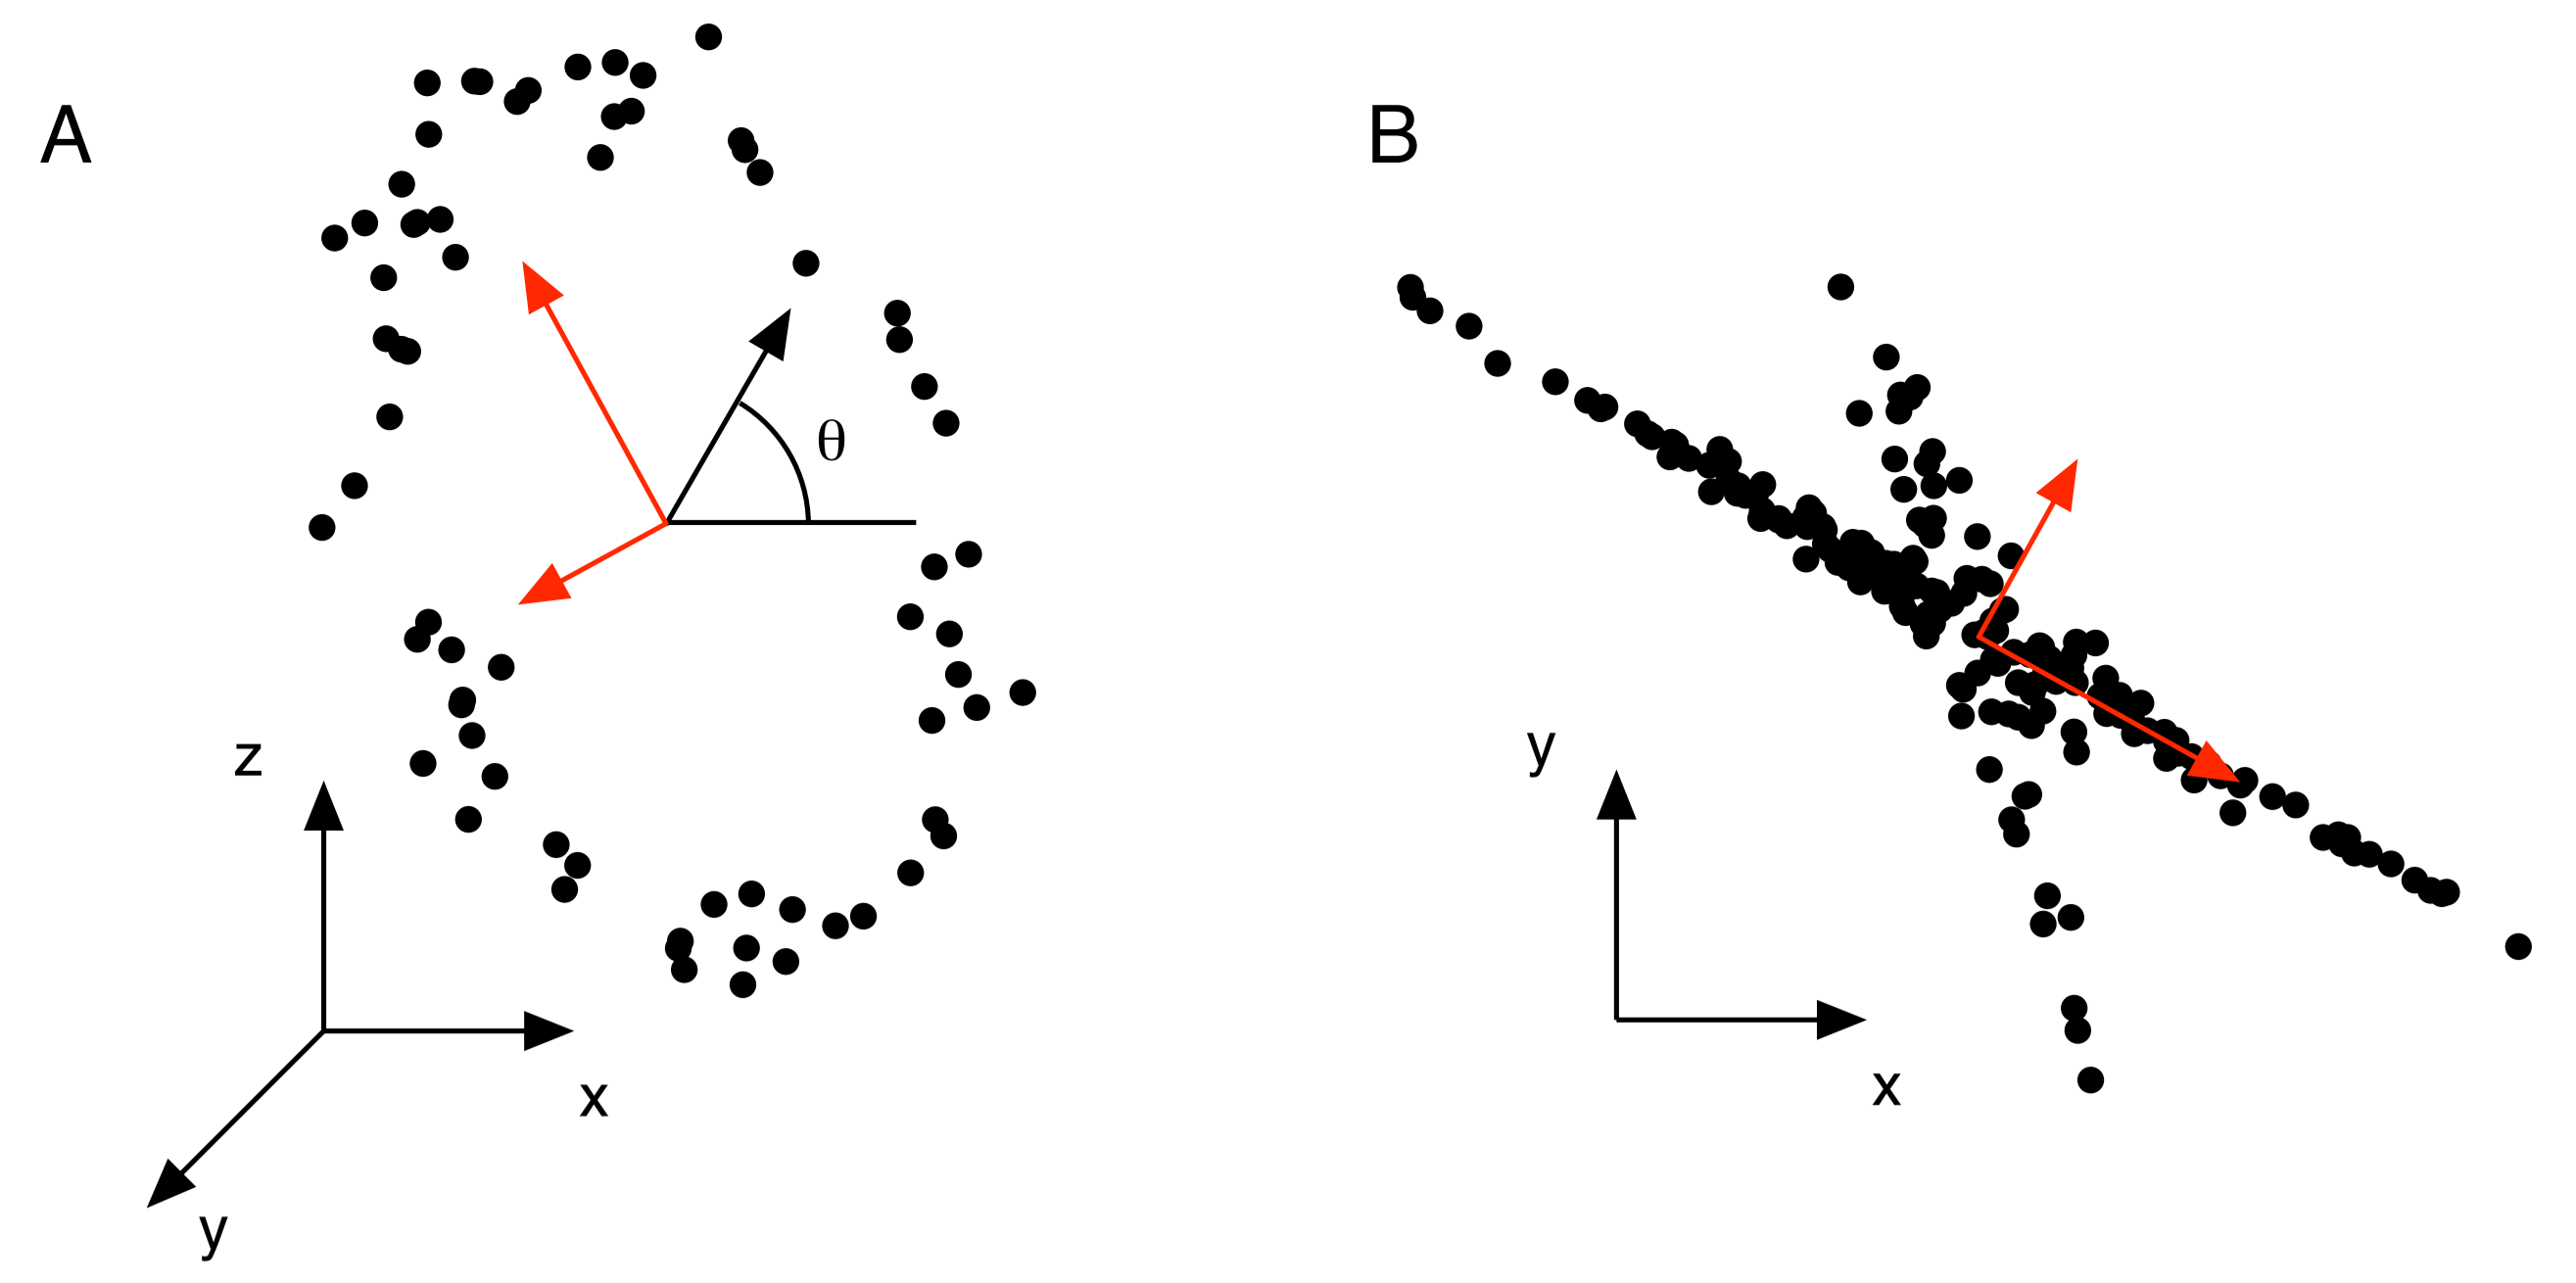
\includegraphics[width=0.8\textwidth]{figures/PCAdifficulties.png}
    \caption{Caption\cite{PCAshlens2014tutorial}}
    \label{fig:pcadifficulties}
\end{figure}

To be able to get accurate results, a \gls{pca} would be sufficient if the dense subclusters had either only a single linear correlation or almost orthogonal ones. However the density-based clustering in step 1 cannot guarantee this property since it can detect arbitrary shapes. This means, that there could be constellations of points which would heavily skew the results of \gls{pca} (c.f.~\autoref{fig:pcadifficulties})\cite{PCAshlens2014tutorial}. 

Since \gls{4c} is basically looking for dense clusters with a biased distance function first and then applying \gls{pca} it has the same disadvantages as \gls{pca} itself~\cite{4cbohm2004computing}. Our whole subcluster already is defined as dense by the previous step and therefore \gls{4c} is prone to also label the whole subcluster as (correlation) dense too and to just consider the whole subcluster as its target. Hence applying \gls{pca} afterwards equals to the application of only \gls{pca} onto the whole subcluster. 
\gls{orclus} is also not suited well. It performs a $k$-means like approach first to partition the subcluster~\cite{orclusaggarwal2000finding}, however since our density-based preprocessing step finds different arbitrary shapes, which implies a different number of correlations, in each clusterpartition, choosing a meaningful $k$ is difficult or impossible. \todor{soll der teil in related work? Moechte den als uebergang benutzen um die Verwendung von CASH zu begruenden}
Compared to \gls{orclus} and \gls{4c}, \gls{copac} has better capabilities of finding correlation clusters, but lacks in the ability to find a generalized view, e.g. it would not identify two intersecting lines in a 3-dimensional space as a possible hyperplane, but as two lines. 

To cover this scenario as well, we choose to adopt \gls{cash}, which does not rely on the clusters eigenvectors, is resistant to noise and outliers, and creates an accurate view of a subspace with a requested dimensionality.

After finding all dense regions of interest, the subclusters are independently evaluated for their local correlations without considering the other points in data space. This is done by applying the \gls{cash} algorithm onto the locally dense clusters. \gls{cash} transforms each point of the cluster into the parameter space and splits it according to its parameters minimum Points $m$ and number of splits $s$ as discussed in \autoref{ssec:CASHindepth}. The resulting correlations are then bounded by the region of interests intervals (bounding box), which represent the local subspace clusters in the dense region.

\subsection{Stitching}

To combine the localized correlations to a global correlation clustering, we evaluate all the localized correlations without its bounding boxes. Since we can represent the localized correlations as hyperplanes with a unit normal vector $\vec{n}$ and a shortest distance to origin $\delta$ (c.f. \autoref{eq:highhnf}), we can easily compare different hyperplanes by variation in rotation(angles), using the cosine-similarity between the normal vectors, and translation(absolute positioning), using the euclidean-distance between the shortest distances. For adjustability we introduce two parameters $thres_{\Delta \text{cos-dist}}$ and $thres_{\Delta \text{eudl-dist}}$, which serves as thresholds for maximal allowed divergence of both measures. To formalize the requirements for a successful combination (\textit{stitching}) of local correlations we introduce following relations:

\subsubsection*{Orientation-Similarity}
Given a set of unique linear correlations $C$ in \gls{hnf}. Then two correlations $a \in C$ and $b \in C$ are \textit{orientation-similar}, if the absolute cosine-similarity between $a$ and $b$ is bigger than $1 - thres_{\Delta \text{cos-dist}}$.
\begin{align}
    cos-sim(a,b) = \frac{\sum_{i=1}^{n} a_{i} b_{i}}{\sqrt{\sum_{i=1}^{n} a_{i}^{2}} \sqrt{\sum_{i=1}^{n} b_{i}^{2}}} >
\end{align}

\chapter{Evaluation}
To measure the performance of our algorithm, we evaluated \todor{werden tests evaluiert, oder algorithmen?} it on custom synthetic \textit{labeled} data sets, generated via the method mentioned in \autoref{sec:datagen}, which serves as the \textit{groundtruth} of our data. Explicitly we compared our novel algorithm with its ancestor \gls{cash} in clustering and runtime performance in various settings we will mention later. Since clustering is an unsupervised setting and the different clustering algorithms do not label the clusters uniformly with the same schema/value, we chose to compare the clustering labels via the \gls{ari}\cite{hubert1985comparingari} and \gls{nmi}\cite{strehl2002clusternmi} score, which are invariant to the permutations of the labeling. Later in this chapter we review the available hyperparameters of our algorithm and, based on previously evaluated data, explain their impacts on the performance.

The algorithms and evaluation are implemented in \textit{python v3.7.4}. Each of the data sets locally dense correlations are uniquely labeled and previously pruned noise points relabeled to a nearby linear correlation if the point was within a certain vicinity from the correlation away. For the density-based clustering we applied \gls{optics} from \textit{scikit-learn v0.21.2}\cite{pedregosa2011scikit} and for the extraction of the correlations we utilized \gls{cash} from the data mining tool \textit{\gls{elki} v0.7.5}\cite{achtert2008elki}. 

% We defined the threshold of the vicinity as $jitter_{thres}$ which merges the noise points if the euclidean distance to a nearby linear correlation $distance_{point\rightarrow hyperplane} = \frac{\Vec{n}\cdot\Vec{x}+\delta}{|\Vec{n}|}$ is smaller than the threshold. These data sets are served as our \textit{groundtruth}. Based on these groundtruths we compared our local-global combining clustering approach's results with its ancestor \gls{cash}'s results in the accuracy of their labeling based on the \gls{ari} and \gls{nmi} score and its runtime performance.

\todor{reichen 2d veranschaulichungen? 3d is hard}

\section{Setup}\label{sec:setup}

Our test setups were conducted on $d$-dimensional synthetic data sets with four characteristic jittery $d-1$-dimensional correlations, i.e. partial, intersecting and/or parallel correlations. The tests consisted of the evaluation of the algorithms different behaviours w.r.t runtime, \gls{ari} and \gls{nmi} scoring for six different amounts of points/objects (1000, 2000, 4000, 8000, 16000, 32000), five different dimensionalities (2, 3, 4, 8, 16) and seven different levels of noise (0, 1, 5, 10, 25, 40, 80).

All following tests were executed in docker containers running on a Virtual Machine with an x86\_64 bit architecture, 48 CPUs (2 GHz) and 246GB RAM. 

\begin{figure}
    \centering
    \begin{minipage}[t]{.5\textwidth}
    \centering
    \captionsetup{width=.9\linewidth}
    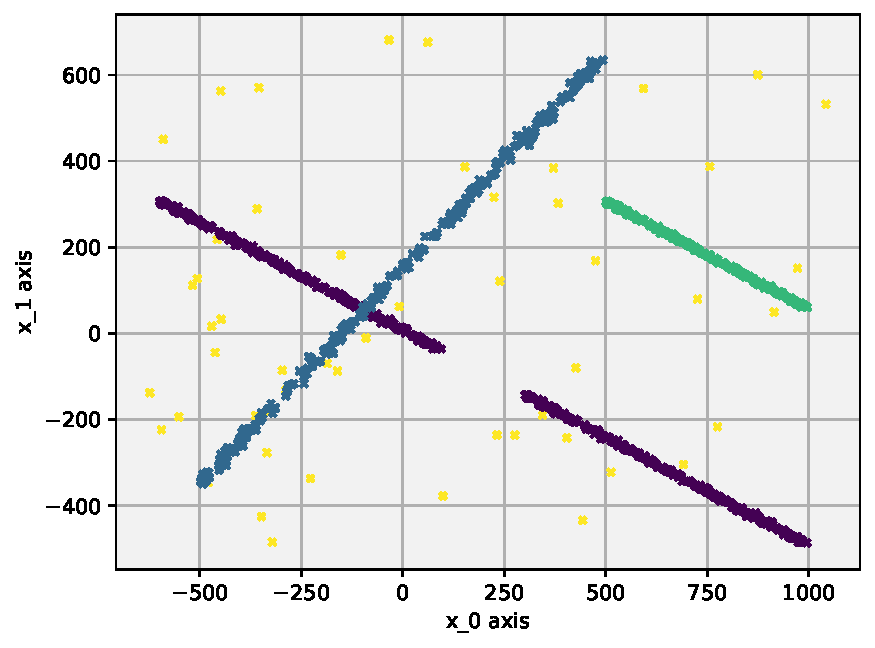
\includegraphics[width=\textwidth]{evalfigures/2DSetGrid.pdf}
    \captionof{figure}{Insight into clustering structure in 2D and 3D}
    \label{fig:my_label}
    \end{minipage}%
    \begin{minipage}[t]{.5\textwidth}
    \centering
    \captionsetup{width=.9\linewidth}
    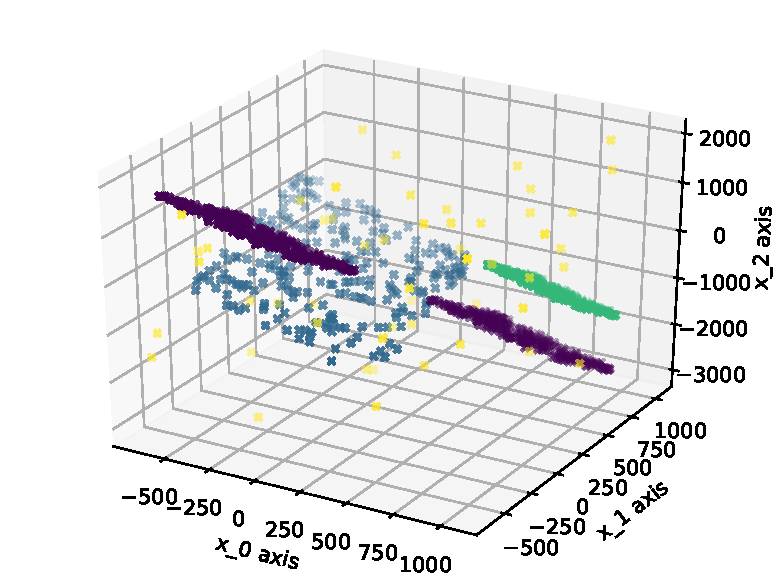
\includegraphics[width=\textwidth]{evalfigures/3DSet.pdf}
    \captionof{figure}{Insight into clustering structure in 2D and 3D}
    \label{fig:my_label}
    \end{minipage}%
\end{figure}

% The algorithms and evaluation are implemented in \textit{python v3.7.4}. Each of the data sets locally dense correlations are uniquely labeled and previously pruned noise points relabeled to a nearby linear correlation if the point was within a certain vicinity from the correlation away. For the density-based clustering we applied \gls{optics} from \textit{scikit-learn v0.21.2}\cite{pedregosa2011scikit} and for the extraction of the correlations we utilized \gls{cash} from the data mining tool \textit{\gls{elki} v0.7.5}\cite{achtert2008elki}. 

% (which data sets have been used? How many data objects? How many clusters? Which programming language and libraries? On which hardware?) [0.5]
\section{Performance}
 To evaluate the performance of our algorithm compared to \gls{cash} we performed up to 500 iterations of random parameter search on each data set while tracking runtime for a measure of efficiency and scoring the effectivity based on the \gls{ari} and \gls{nmi} score compared to our prelabeled groundtruth. However due to time constraints we bounded the maximal time for all iterations to a maximum of 24 hours. \todor{unsicher ob das rein soll}We’d like to note at this point that the current implementation may not satisfy the need to deliver a high performance with regards to the runtime, since we rely on \gls{elki}, which temporarily stores our necessary intermediate results to disk and therefore bottlenecks on I/O. For future work, we recommend to further research and elaborate on strategies to accelerate the execution time of our approach. 
 
\begin{table}[hb]
\centering
\resizebox{\textwidth}{!}{%
\begin{tabular}{@{}llll@{}}
\toprule
Test setting           & Dimensions & Noise in \% & \# of objects \\ \midrule
Increasing objects    & 3D         & 5           & -             \\
Increasing dimensions & -          & 5           & 10000         \\
Increasing noise      & 3D         & -           & 10000         \\ \bottomrule
\end{tabular}%
}
\caption{}
\label{tab:reducedsetup}
\end{table}
 
\subsection{Efficiency}
In context of efficiency we investigate the runtime performance of both local (our algorithm) and global (default \gls{cash}) by three different indications, namely number of objects, number of dimensions and amount of noise.

For the first aspect, we increased the data sets with regards to the number of objects. Here, we asked deliberately: what is the impact regarding the runtime if we modify the data set size?
And further: do we observe any differences between the original \gls{cash} algorithm and our approach? In theory we expect that our method yields similar results as \gls{cash}.

%  The evaluation of runtime performance measures the average runtime of the three different settings for both local (our algorithm) and global (default \gls{cash}) approaches. 

\begin{figure}[h]
    \centering
    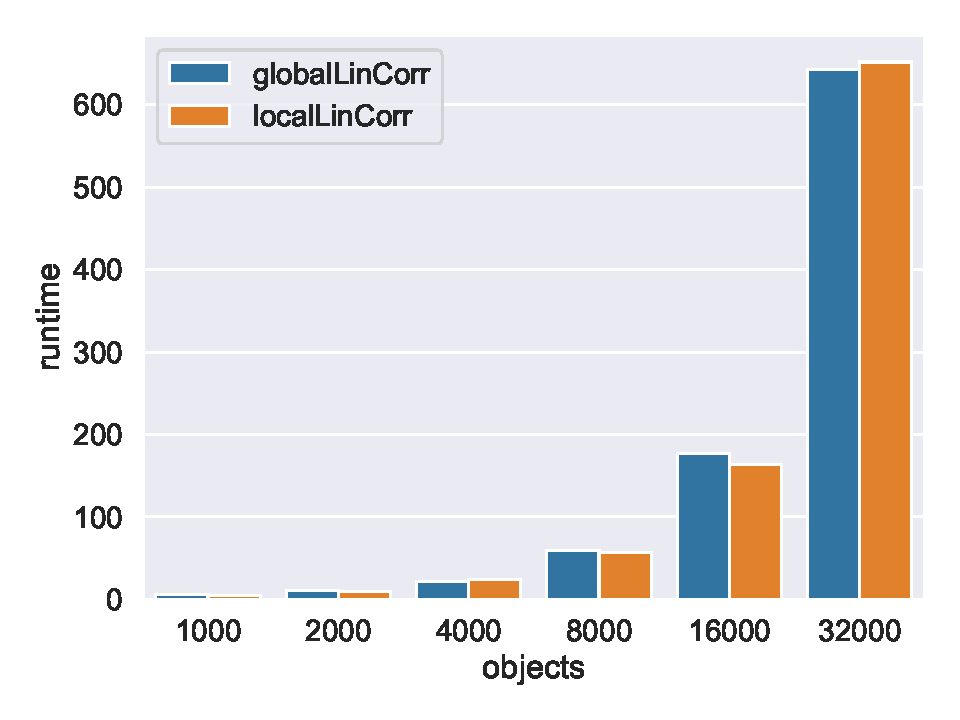
\includegraphics[width=0.8\textwidth]{evaluation/per_objects/Avg_Runtime_3D_N5_pobjects_bar.pdf}
    \caption{Caption}
    \label{fig:eval_per_objects}   
\end{figure}

\autoref{fig:eval_per_objects} shows the average runtime of both algorithms w.r.t. the \textit{number of objects} in 3-dimensional clusters of the data set. The data sets had a variable size of 1000, 2000, 4000, 8000, 16000 and 32000 number of objects with 5 percent noise respective to the data set size. Here our algorithm scales comparably to \gls{cash} and does not deteriorate in runtime performance even with higher numbers of objects even though the overhead of the partitioning, stitching and relabeling increases. This can be explained due to the shorter runtimes of the localized \gls{cash} processes, since the partitioning step reduces the amount of regions of interest in the parameter space of the Hough transform.\\

The second question regarding to efficiency is: How fast does our algorithm perform at different levels of noise? Is it comparable to the original \gls{cash}?. To assess the robustness of our algorithms efficiency against noise we compared the average runtimes of 500 iterations of both algorithms with respect to the amount of noise in the data space. Instead of modifying the total number of points of the whole data set, we now just evaluate the impact of different levels of noise percentage and compare the results of our approach with \gls{cash}s.

% of the average runtime w.r.t the different dimensionalities of the data space is depicted in \autoref{fig:eval_per_dim}.

\begin{figure}[h]
    \centering
        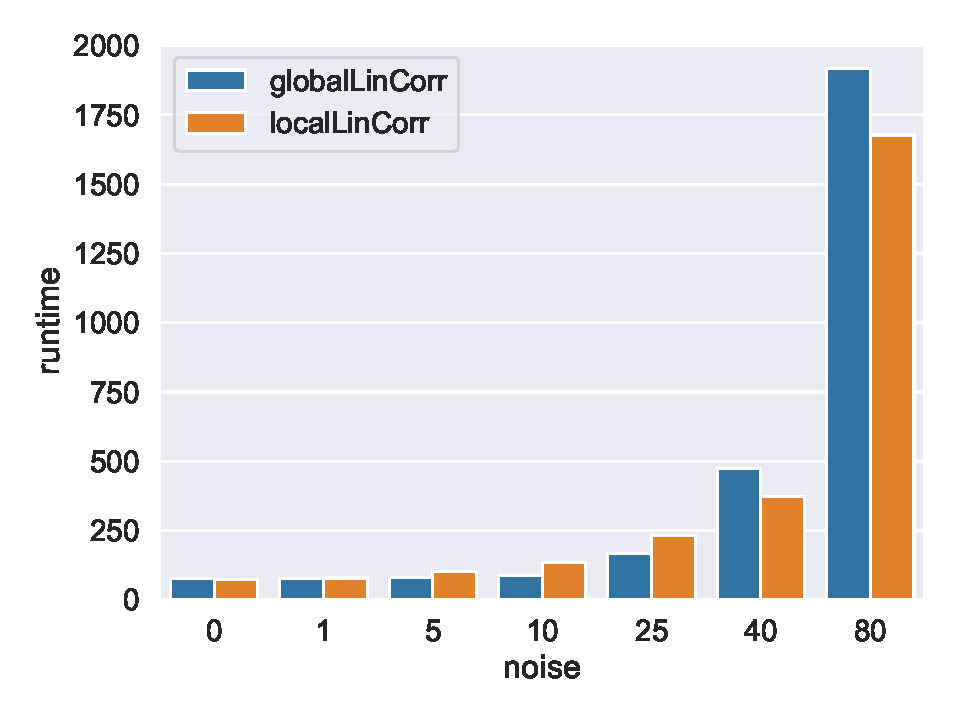
\includegraphics[width=0.8\textwidth]{evaluation/per_noise/Avg_Runtime_3D_O10000_pnoise_bar.pdf}
    \caption{Runtime in seconds w.r.t. the noise percentage}
    \label{fig:eval_per_noise}
\end{figure}

\autoref{fig:eval_per_noise} shows the average runtime of our algorithm with respect to the noise percentage of the data sets compared to the global approach. In this experiment our algorithms were evaluated on a 3-dimensional data set with 10000 points distributed among all clusters and seven different levels of noise percentage (0,1,5,10,25,40,80) on top of the initial data set. Note that noise points close enough to existing correlation clusters are relabeled to the respective cluster before evaluation which slightly skews the actual noise percentage in each data set.
As in the previous runtime measurements with regards to number of objects, the runtimes with respect to noise also remain stable on multiple levels compared to the global \gls{cash}. The overhead of the other components again is compensated by the quicker runtime of the partitioned \gls{cash}. At higher levels of noise (40 and 80 percent) it is even noticeable, that our approach gets a slight speed up compared to the global approach, since at these levels of noise the global cash will need to process more candidates in parameter space. In comparison our approach prunes away density-based noise first due to the partitioning step and leaves each localized \gls{cash} with comparably less candidates.
% At very low levels of noise both algorithms runtime remain stable. However increasing the noise further creates a gap in runtime results in favor of the global approach. This might be due to the overhead of the components increasing faster compared to the reduction in runtime of \gls{cash}, and second 

Our last runtime evaluation was conducted with regards to the dimensionality of the data set. Unlike in previous experiments, the data sets now change in \textit{space} instead of number of data objects. To keep a consistent comparable setting between the dimensionalities, we enforce our data set to be composed of similar four characteristic correlations, building a data space with partially split, intersecting and parallel $d-1$-dimensional hyperplanes. 
Note that runtimes dependent on dimensionality scale in $\mathcal{O}(2^d)$. Therefore the runtime figure with respect to the dimensionality scales logarithmically on the y-axis. Due to time constraints we set an upper bound for the runtime and restricted each run to a maximum of two hours. \todor{soll das rein?}

\begin{figure}[h]
    \centering
        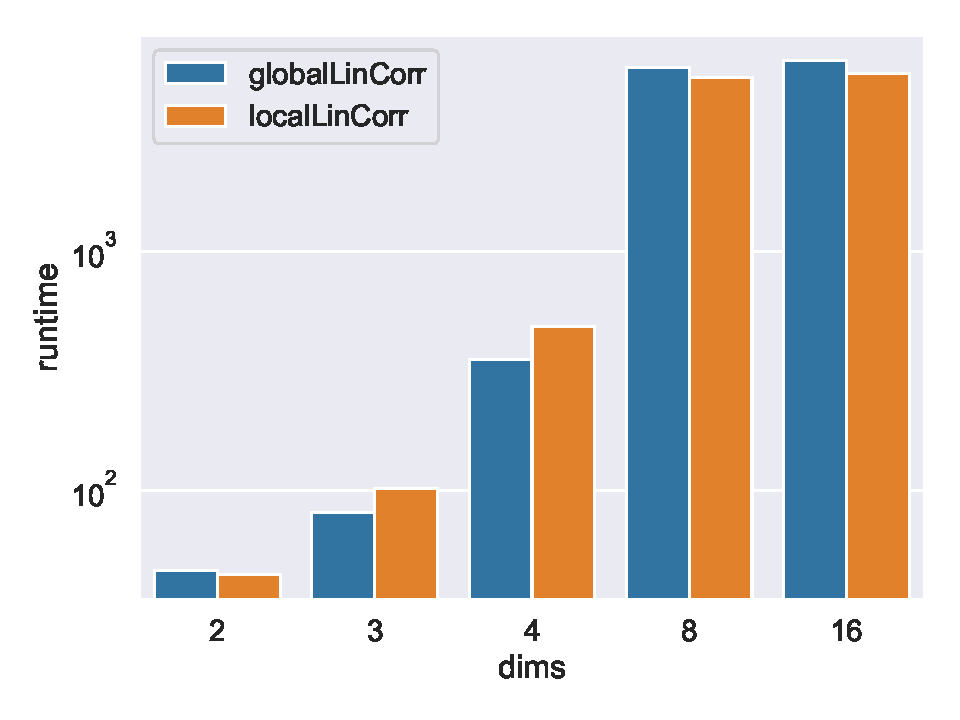
\includegraphics[width=0.8\textwidth]{evaluation/per_dims/Avg_Runtime_O10000_N5_pdims_log.pdf}
    \caption{Runtime in seconds w.r.t. the dimensionality of the whole data set - lower is better}
    \label{fig:eval_per_dims}
\end{figure}

\autoref{fig:eval_per_dims} shows a comparison of local and global algorithms average runtime performances with regards to expanding dimensionalities. This experiment was ran on data sets with 10000 objects and 5 percent noise with 2,3,4,8 and 16 dimensions. As expected the average runtime corresponding to the increasing dimensionality increases exponentially for both approaches, considering the runtime complexity of \gls{cash} and our algorithms complexity, which is also dominated by the complexity of \gls{cash}s $\mathcal{O}(2^d)$. Therefore it is sensible that both algorithms again perform comparably.
Since we capped the maximum runtime of each parameter search iteration to 2 hours we observe a stagnation of the runtime at 16 dimensions.\\

Summarized the experiments have demonstrated that the average runtime of our local approach is closely comparable to the default \gls{cash} with respect to number of points, amount of noise and dimensionalities. Therefore as assumed the overhead produced by the preprocessing component \gls{optics} and the postprocessing components \textit{Stitching} and \textit{Relabeling} are compensated by the faster runtime of the localized \gls{cash} ran on the partitioned subinterval of the data space. 
 
\subsection{Effectiveness}
To measure the clustering performance measures we picked the best parameter sets of the previous 500 iterations of parameter search of the efficiency evaluation for both local and global approach and stacked their \gls{ari} and \gls{nmi} scores up against each other. 

In our first setting we compared \gls{cash} and our algorithm according to the best \gls{ari} and \gls{nmi} scorings achieved during the parameter search with regards to the variable number of objects in data space. 
\begin{figure}[h]
    \centering
    \begin{minipage}[t]{.5\textwidth}
      \centering  
      \captionsetup{width=.9\linewidth}
      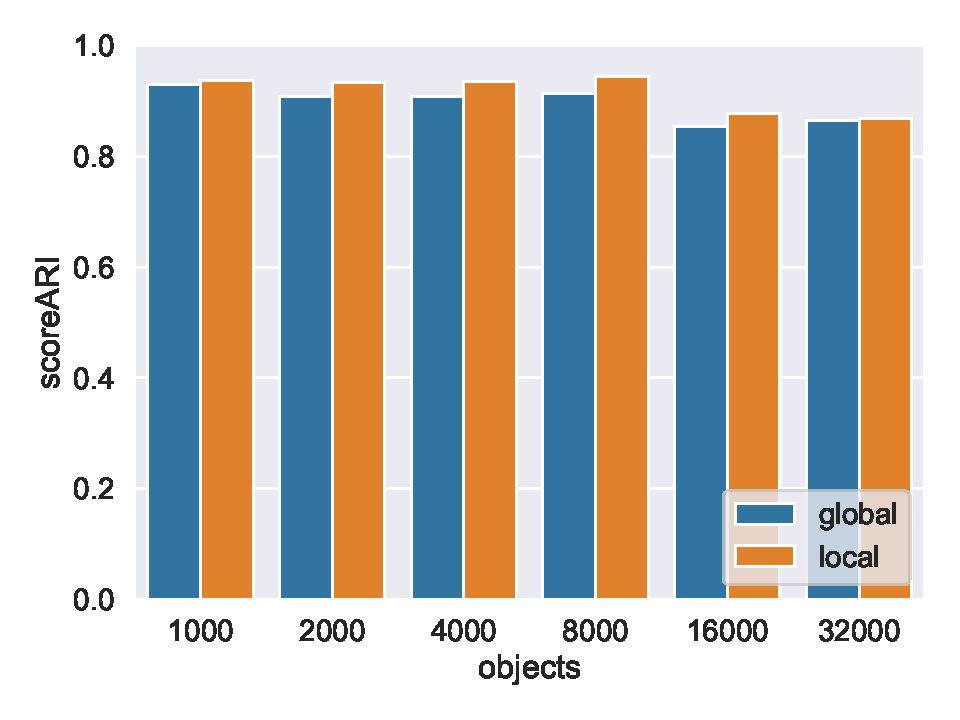
\includegraphics[width=\textwidth]{evaluation/per_objects/Best_ARI_3D_N5_pobjects_bar.pdf}
      \captionsetup{labelformat=empty}
      \caption{\gls{ari} score}
      \label{fig:ariperpts}
    \end{minipage}%
    \begin{minipage}[t]{.5\textwidth}
      \centering
      \captionsetup{width=.9\linewidth}
      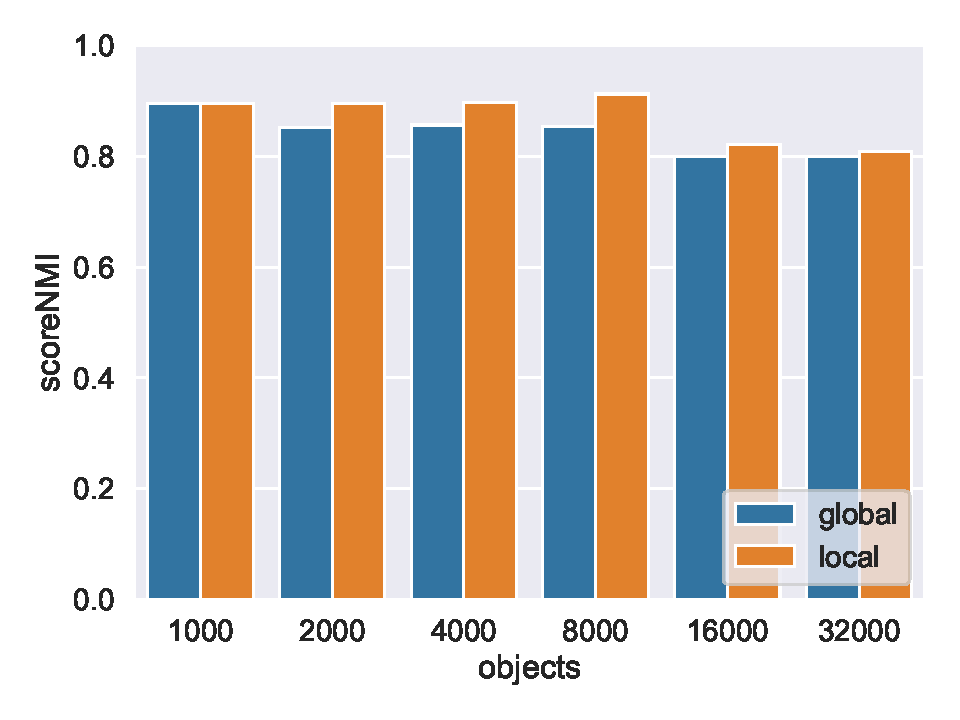
\includegraphics[width=\textwidth]{evaluation/per_objects/Best_NMI_3D_N5_pobjects_bar.pdf}
      \captionsetup{labelformat=empty}
      \caption{\gls{nmi} score}
      \label{fig:nmiperpts}
    \end{minipage}
    \caption{Scoring w.r.t the number of objects - higher is better}
    \label{fig:scoreperpts}
\end{figure}

\autoref{fig:scoreperpts} shows the comparison of the clustering scores achieved by both the local and global approach on the 3-dimensional data set with 5 percent noise with respect to six variable numbers of objects (1000, 2000, 4000, 8000, 16000, 32000). In terms of cluster size both algorithms perform comparably and score a similar \gls{ari} and \gls{nmi} score of over $0.8$. 

To assess the robustness of our clustering algorithm against noise, the second clustering performance evaluation was conducted on a data set with variable levels of noise. Given the best parameter settings achieved during the 500 iterations of parameter search in the efficiency evaluation step, we compared the \gls{ari} and the \gls{nmi} scores at different levels of noise of both algorithms against each other.
\begin{figure}[h]
    \centering
    \begin{minipage}[t]{.5\textwidth}
      \centering  
      \captionsetup{width=.9\linewidth}
      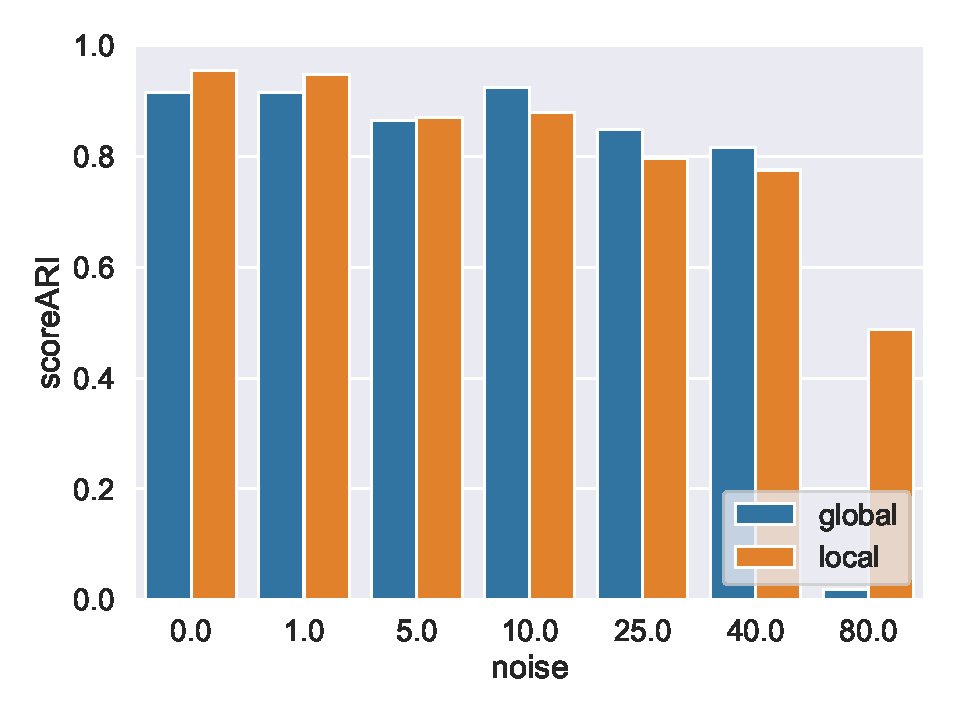
\includegraphics[width=\textwidth]{evaluation/per_noise/Best_ARI_3D_O10000_pnoise_bar.pdf}
      \captionof{figure}{\gls{ari} score w.r.t. amount of noise}
      \label{fig:ariperpts}
    \end{minipage}%
    \begin{minipage}[t]{.5\textwidth}
      \centering
      \captionsetup{width=.9\linewidth}
      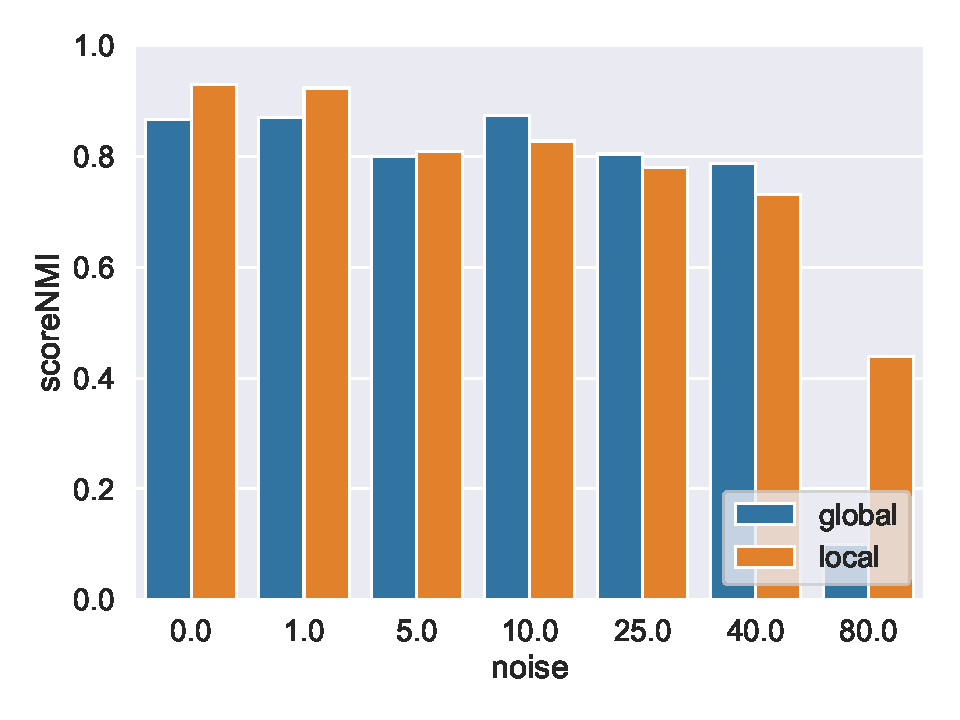
\includegraphics[width=\textwidth]{evaluation/per_noise/Best_NMI_3D_O10000_pnoise_bar.pdf}
      \captionof{figure}{\gls{nmi} score w.r.t. amount of noise}
      \label{fig:nmiperpts}
    \end{minipage}    
    \caption{Scoring w.r.t the noise percentage - higher is better}
    \label{fig:scorepernoise}
\end{figure}
The second experiment was ran on 3-dimensional base data sets with 10000 data points spread among all clusters with seven varying amounts of noise (0,1,5,10,25,40,80).
As \autoref{fig:scorepernoise} shows, the results of the clustering performance evaluation scoring between our algorithm and \gls{cash} remains close to eachother for low to mid levels of noise. At 80 percent noise our algorithm performs even better than the global \gls{cash}. This could be due to the high percentage of noise creating a high amount of candidate cells in parameter space, which are all considered as valid correlations in the global \gls{cash}. In contrast our approaches preprocessing via \gls{optics} might extract the underlying correlations, which are characterized by comparably more dense regions, first and and extract those local correlations via \gls{cash} faster and more accurately, since the partitions contain less noise and therefore the parameter space less candidates. These few prominent local correlations are then stitched together if similar enough and previously not considered points are relabeled, all together resulting in an quicker and more accurate global clustering compared to default \gls{cash} itself.

Our last clustering performance evaluation was targeted at the impact of the dimensionality of the data set. Here, we again picked the best parameter sets previously obtained during the runtime assessment to compare our algorithm with \gls{cash}.
\begin{figure}[h]
    \centering
    \begin{minipage}[t]{.5\textwidth}
      \centering  
      \captionsetup{width=.9\linewidth}
      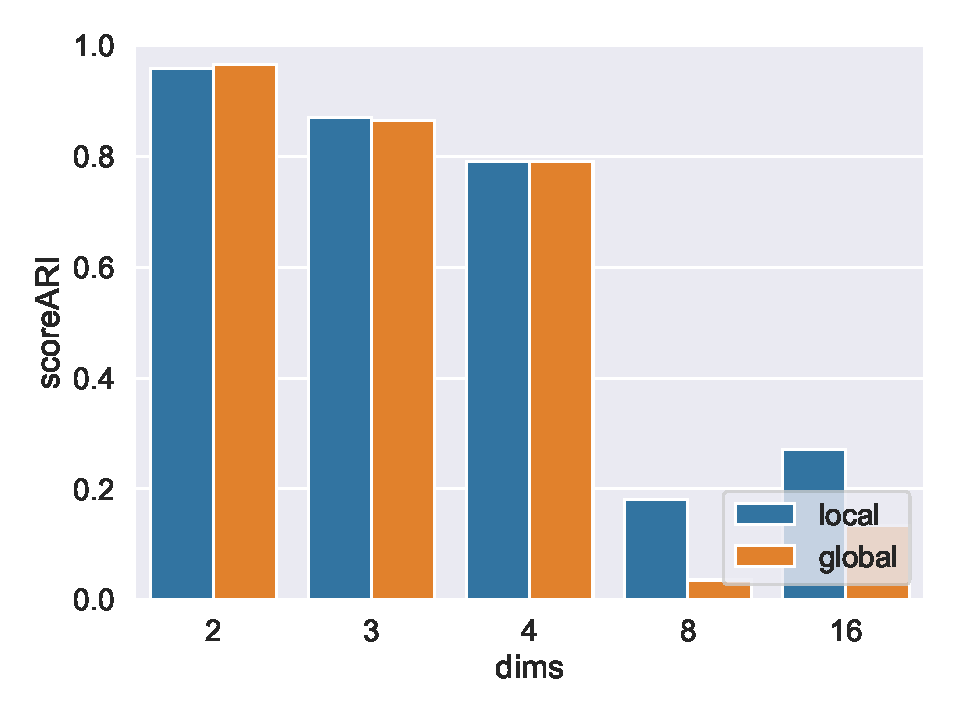
\includegraphics[width=\textwidth]{evaluation/per_dims/Best_ARI_O10000_N5_pdims_bar.pdf}
      \captionof{figure}{\gls{ari} score w.r.t. dimensionality}
      \label{fig:ariperpts}
    \end{minipage}%
    \begin{minipage}[t]{.5\textwidth}
      \centering
      \captionsetup{width=.9\linewidth}
      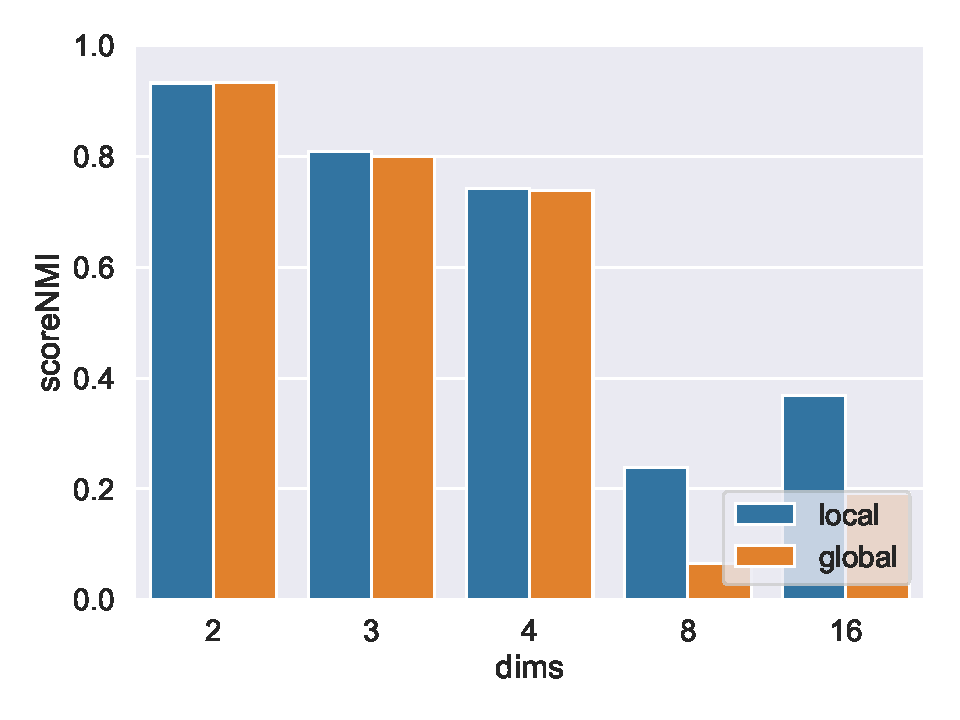
\includegraphics[width=\textwidth]{evaluation/per_dims/Best_NMI_O10000_N5_pdims_bar.pdf}
      \captionof{figure}{\gls{nmi} score w.r.t. dimensionality}
      \label{fig:nmiperpts}
    \end{minipage}
    \caption{Scoring w.r.t the dimensionality - higher is better}
    \label{fig:scoreperdims}
\end{figure}

\autoref{fig:scoreperdims} shows the different scores, \gls{ari} and \gls{nmi}, between both global and local approach applied on data sets with a fixed amount of 10000 data objects and 5 percent noise and a variable dimensionality of 2,3,4,8 and 16.
Note that since the evaluation of the runtime performance with regards to 8 and 16 dimensional data sets were stopped early due to time constraints, the optimal scorings of both 8 and 16 dimensional data sets are not representative for the optimal scores and will not be considered. 
The results of dimensions 2,3 and 4 show similar clustering results compared to both algorithms, however as the direction over these dimensions \gls{ari} and \gls{nmi} scores suggest, both \gls{cash} and our algorithm have an downwards trend in terms of clustering score with regards to dimensionality. This might be due to the fact, that the search space for \gls{cash} increases exponentially with respect to the dimensions, which increases the possible regions of interest (c.f. \autoref{fig:cash3d}). Instead of a single intersection in a point as a region of interest in 2-dimensional space, a 3-dimensional space for comparison has a complex curve as intersection which increases the amount of regions of interest considerably. This increased complexity might be the reason for the deteriorating performance in increasing dimensions. \todor{erwaehnt orginal cash das deswegen nicht?}\\

Summarized our experiments show, that our local approach yields similar results in various settings in terms of runtime as well as in terms of clustering performance compared to the original \gls{cash}, with an additional benefit of detecting locally dense correlations. \autoref{fig:clusterexample} shows an example of our algorithm with the local correlations clustering as an intermediate result and the relabeled global view of the correlation clustering. \autoref{fig:gclusterexample} shows the equivalent clustering performed by the default \gls{cash}. \todor{kann laenger sein}

\begin{figure}
    \centering
    \includegraphics{}
    \caption{Caption}
    \label{fig:clusterexample}
\end{figure}

\begin{figure}
    \centering
    \includegraphics{}
    \caption{Caption}
    \label{fig:gclusterexample}
\end{figure}

% \section{Parameters available and their impacts}
% As our algorithm depends on many components such as \gls{optics} and \gls{cash} which come with several parameters themselves. In this section we discuss their meaning and their impact for the clustering results.

% \subsection{Metrics: CosineSimiliarity(n1,n2), CosineSimiliarity(n1,n2) + EuclidianDistance(d) [2-3]}

% \subsection{Median vs.  Mean}

% \section{Results between Dense approach with stitching and Global approach}

% \section{Test on real world data set(s) [1]}

% %evtl. "Hyperparameter sensitivity" d.h. wie 'empfindlich' ist das verfahren bzgl. welchen Parameter Einstellungen?
\chapter{Conclusion}\label{ch:conclusion}
% Possible improvements by sampling (see \cite{opticsankerst1999optics})
In the present state of huge amounts of data acquisition in various fields,  such as medicine, economy and artificial intelligence, the task of detecting and extracting relevant subspace clusters continues to be highly relevant. However, the current implementations of correlation clustering algorithms only focus on the detection of either local correlation clusters or global correlation cluster and lack the means to find an agglomerated view of both during a single evaluation run. In this thesis, we reviewed existing Correlation Clustering approaches and highlighted their shortcomings concerning their target scope being only applicable for either local or global Correlation Clustering. 

As a solution, we proposed a novel approach for finding both scopes of clustering simultaneously by applying a density-based preprocessing step first and performing a Correlation Clustering algorithm on the resulting locally dense clusters afterwards. This intermediate result contains the local correlation clusters, which represents the local view of the Correlation Clustering. To create the global view, we combined the intermediate clusters by stitching them together if they are similar enough and relabelled all previously disregarded (not dense) points for completeness.

% Our empirical performance analysis in terms of clustering accuracy and runtime was conducted on three different experiments with regards to variable numbers of data objects, amounts of noise and dimensionalities, and additionally compared to the performance measures of its parent algorithm \gls{cash}.
To evaluate the performance in terms of clustering accuracy and runtime, we conducted three different settings for experiments with regards to the number of data objects, amount of noise and dimensionality, and compared those to the performance measures of its parent algorithm \gls{cash}. 
The runtime results yielded that on average, our algorithm, in each runtime setting, performs comparably to \gls{cash} and even gets a slight edge at a comparison in high noise levels. With regards to higher dimensionalities however, we were not able to retrieve representable performance measures due to time and processing power constraints. In terms of clustering performance, our tests, with the best parameter setting previously determined, revealed similar clustering scores as well, with our algorithm having an advantage at higher levels of noise again. However, the tests on the dimensionality also exposed, that both algorithms scale worse for increasing dimensions. At high dimensions, our algorithms best score paled in comparison to \gls{cash} due to the best parameter set being harder to determine since our algorithm requiring more parameters.

All things considered, our first empirical performance analysis yields that, in addition to providing both local and global Correlation Clustering, our algorithm performs equally well compared to original \gls{cash} in terms of the global view, and suggests promising performance in regards to correlation clusterings with arbitrary scopes.

\chapter{Future Work}\label{ch:futurework}
As the topic of correlation clustering with arbitrary scopes is by no means covered and is just at the beginning of the research, we want to provide suggestions for an outlook of potential future directions. 
% To provide an outlook of potential future directions gathered by ideation during the process of the creation of this work, we hope to motivate for future research and present the following contributions.

This work only covered a basic principle of assembling locally dense clusters with global correlation clustering via \gls{dbscan}/\gls{optics} and \gls{cash}. However, these components only served as quick and convenient building blocks to realize an implementation of said principle and by no means have to be the optimal solutions. For future work, we suggest to research and experiment with different, more advanced or modified components, e.g. using modified distance functions in \gls{dbscan}/\gls{optics} to cope for the Curse of Dimensionality, choosing a different Correlation Clustering method for improved correlation results or modifying the assembling method of the local correlation clusters.

As the in-depth evaluation of the impact to the performance measures for every single parameter is very extensive and was not possible in the frame of this thesis, a survey about the different parameters and their impacts with regards to local and global clustering results could be subject to future research.

Another path of future work targets the implementation of our algorithm itself as our work does not satisfy the need for high performance with regards to runtime we recommend to further research and elaborate on strategies to accelerate the execution time of our approach.



\appendix
\chapter{Synthetic Data Generation}
\label{sec:datagen}
For the sake of completeness and for testing purposes we created a generator of (random) data sets containing variable linear correlations and noisepercentages.

The generation of n-dimensional linear correlations is done in four steps:
\begin{enumerate}
\item Generation of random unit normal vectors and distances for the \acrfull{hnf}: 
\begin{align}
\text{dimension }d&: \text{number of dimensions of data set}\\
\text{unit normal vector } \vec{n}&: (n_0, \cdots, n_d )^T, n_i \in \mathbb{R} \text{ and } |\vec{n}| = 1\\
\text{distance }\delta&: \delta \in \mathbb{R}
\end{align}
\end{enumerate}

These parameters define the orientation of the linear correlations and can be set randomly or manually.

\begin{enumerate}[resume]

\item Create HNF and solve by last dependent dimension:
\begin{align}
    \text{HNF}: \vec{n} \cdot \vec{x} = n_0 * &x_0 + \cdots + n_d * x_d = \delta, x_i \in \text{Set of Dimensions}\\
    \begin{split}
        \text{last Dim}: x_{lastDim} &= f(x_0, \cdots, x_{k}) \\
        &= \frac{a_0 * x_0 + \cdots + a_{k} * x_{k}}{a_{lastDim}}, i \in \{1,\dotsc,d\}\setminus {lastDim}
    \end{split}
\end{align}
\end{enumerate}

Since we want to generate arbitrarily oriented linear correlations, we cannot simply expect dimension $d$ to be dependent on the dimensions $d_i, d_i < d$, since axis-parallel linear correlations have dimensions not dependent on others. Therefore we need to analyze the normal vector first and base our point generator on the vectors orientation.

\begin{enumerate}[resume]

\item Generate points with $k$ dimensions to calculate their lastDim according to the HNF and stack them together.
\begin{align}
    \text{randomPt}&: tmp = (v_0, \cdots, v_{k}), tmp \in \mathbb{R}^{k}\\
    \text{linCorrPt}&: corrPts =  (v_0, \cdots, v_{k}, f(tmp)), corrPts \in \mathbb{R}^{d}
\end{align}
\end{enumerate}



\begin{enumerate}[resume]
\item Generate noise and attach it to working dataset:
\begin{align}
    \text{noisePts}: noise = (w_0, \cdots, w_d), noise \in \mathbb{R}^{d}
\end{align}
\end{enumerate}

The generation of all points, be it linear correlated points or noise points can be drawn from a arbitrary distribution $X \sim pdf(x)$, e.g. normal distribution $X \sim \mathcal{N}(\mu,\sigma^2)$ or uniform distribution $X \sim \mathcal{U}(a,b)$.

\chapter{Results}

Results with Figures?

% Abbildungsverzeichnis (kann auch nach dem Inhaltsverzeichnis kommen)
% \listoffigures

% \listofalgorithms
% \addcontentsline{toc}{chapter}{List of Algorithms}
% % Tabellenverzeichnis (kann auch nach dem Inhaltsverzeichnis kommen)
% \listoftables

% Literaturverzeichnis
% \bibliographystyle{plainnat}
% \bibliographystyle{dbstmpl}    % verwendet dbstmpl.bst
% % alternative, vorinstallierte Stile sind z.B. plain oder abbrv
% \bibliography{dbstmpl}         % verwendet dbstmpl.bib
\printbibliography

\end{document}
